\documentclass[11pt]{article}
\usepackage[margin=1in]{geometry}
\usepackage{amsmath,amssymb,amsthm,bm}
\usepackage{graphicx}
\usepackage{booktabs}
\usepackage{array}
\usepackage{siunitx}
\usepackage[hidelinks]{hyperref}
\usepackage{xcolor}
\usepackage{caption}
\usepackage{enumitem}
\usepackage{mathtools}
\usepackage[section]{placeins}
\renewcommand{\topfraction}{0.9}
\renewcommand{\bottomfraction}{0.8}
\renewcommand{\textfraction}{0.07}
\renewcommand{\floatpagefraction}{0.8}
\setcounter{topnumber}{3}
\setcounter{totalnumber}{5}

\newcommand{\R}{\mathbb{R}}
\newcommand{\C}{\mathbb{C}}
\newcommand{\dd}{\mathrm{d}}
\newcommand{\Om}{\Omega}
\newcommand{\zall}{\zeta_{\mathrm{all}}}
\newcommand{\UD}{\mathrm{UD}}
\DeclareMathOperator{\Imag}{Im}
\DeclareMathOperator{\Real}{Re}
\DeclareMathOperator*{\argmin}{arg\,min}
\newtheorem{proposition}{Proposition}
\newtheorem{corollary}{Corollary}
\theoremstyle{remark}
\newtheorem{remark}{Remark}

% AUTO-GENERATED by examples/paper_numbers.py -- do not edit by hand.
\newcommand{\nAngFstd}{0.7}
\newcommand{\nAngJmean}{0.365}
\newcommand{\nAngJstd}{0.007}
\newcommand{\nAsBuiltFmax}{1.12}
\newcommand{\nAsBuiltFmin}{0.96}
\newcommand{\nAsBuiltJmax}{0.38}
\newcommand{\nAsBuiltJmin}{0.29}
\newcommand{\nAsBuiltMaxDev}{0.08}
\newcommand{\nAsBuiltMmax}{1.12}
\newcommand{\nAsBuiltMmin}{0.97}
\newcommand{\nBBf}{0.90}
\newcommand{\nBBred}{2}
\newcommand{\nBEighteenHeld}{0.656}
\newcommand{\nBEighteenHeldCond}{0.667}
\newcommand{\nBEighteenHeldRed}{34}
\newcommand{\nBEighteenHeldf}{0.978}
\newcommand{\nBEighteenNinety}{0.440}
\newcommand{\nBEighteenNinetyCond}{0.430}
\newcommand{\nBEighteenNinetyRed}{56}
\newcommand{\nBEighteenNinetyf}{0.896}
\newcommand{\nBInfHeld}{0.405}
\newcommand{\nBInfHeldCond}{0.414}
\newcommand{\nBInfHeldRed}{59}
\newcommand{\nBInfHeldf}{0.976}
\newcommand{\nBInfNinety}{0.375}
\newcommand{\nBInfNinetyCond}{0.370}
\newcommand{\nBInfNinetyRed}{62}
\newcommand{\nBInfNinetyf}{0.916}
\newcommand{\nBNineHeld}{0.813}
\newcommand{\nBNineHeldCond}{0.818}
\newcommand{\nBNineHeldRed}{19}
\newcommand{\nBNineHeldf}{0.979}
\newcommand{\nBNineNinety}{0.621}
\newcommand{\nBNineNinetyCond}{0.627}
\newcommand{\nBNineNinetyRed}{38}
\newcommand{\nBNineNinetyf}{0.898}
\newcommand{\nBUDf}{207.2}
\newcommand{\nBUDrms}{2.06}
\newcommand{\nBUnif}{1.0000}
\newcommand{\nBUnifFFortyFive}{0.561}
\newcommand{\nBUnifFTwenty}{0.895}
\newcommand{\nBeamCondFE}{0.011}
\newcommand{\nBeamFreqBand}{2.4}
\newcommand{\nBeamMaxAngle}{83}
\newcommand{\nCFratio}{1.64}
\newcommand{\nCOptac}{0.347}
\newcommand{\nCOptbetaEPMC}{0.246}
\newcommand{\nCOptbetaSSM}{0.248}
\newcommand{\nCOptepmcSec}{2173}
\newcommand{\nCOptf}{258.3}
\newcommand{\nCOptgap}{0.000}
\newcommand{\nCOptrsix}{0.247}
\newcommand{\nCOptrten}{0.247}
\newcommand{\nCSEleven}{0.74}
\newcommand{\nCSTen}{1.00}
\newcommand{\nCSThirteen}{0.55}
\newcommand{\nCSTwelve}{0.61}
\newcommand{\nCUDac}{0.208}
\newcommand{\nCUDbetaEPMC}{0.680}
\newcommand{\nCUDbetaSSM}{0.689}
\newcommand{\nCUDepmcSec}{2054}
\newcommand{\nCUDf}{256.3}
\newcommand{\nCUDgap}{0.128}
\newcommand{\nCUDrsix}{0.684}
\newcommand{\nCUDrten}{0.684}
\newcommand{\nCacFormOpt}{0.353}
\newcommand{\nCacFormUD}{0.211}
\newcommand{\nCacRatio}{1.66}
\newcommand{\nCacTheory}{1.67}
\newcommand{\nCeil}{0.33}
\newcommand{\nChiBase}{33}
\newcommand{\nChiCl}{27}
\newcommand{\nChiMv}{27}
\newcommand{\nChiSq}{48}
\newcommand{\nChiTwo}{21}
\newcommand{\nConflict}{33}
\newcommand{\nConvBase}{0.37}
\newcommand{\nConvFreqDrop}{0.9}
\newcommand{\nConvThree}{0.52}
\newcommand{\nCratioEPMC}{0.362}
\newcommand{\nCratioSSM}{0.359}
\newcommand{\nCredEPMC}{64}
\newcommand{\nCredSSM}{64}
\newcommand{\nCtsF}{0.42}
\newcommand{\nCtsJ}{100}
\newcommand{\nCtsM}{0.43}
\newcommand{\nDJ}{0.37}
\newcommand{\nDampAcHi}{0.290}
\newcommand{\nDampAcHiOpt}{0.482}
\newcommand{\nDampAcLo}{0.106}
\newcommand{\nDampRatioMax}{1.665}
\newcommand{\nDampRatioMin}{1.663}
\newcommand{\nDampScale}{0.49}
\newcommand{\nDampStiffRatio}{1.69}
\newcommand{\nDetThreeOne}{5}
\newcommand{\nDgamma}{0.38}
\newcommand{\nDknl}{0.52}
\newcommand{\nDmid}{1.01}
\newcommand{\nDomsq}{1.00}
\newcommand{\nDoseA}{0.98}
\newcommand{\nDoseB}{0.94}
\newcommand{\nDoseC}{0.84}
\newcommand{\nDoseD}{0.66}
\newcommand{\nDoseE}{0.37}
\newcommand{\nDoseF}{0.21}
\newcommand{\nDoseRatioA}{1.2}
\newcommand{\nDoseRatioB}{1.7}
\newcommand{\nDoseRatioC}{2.9}
\newcommand{\nDoseRatioD}{5.4}
\newcommand{\nDoseRatioE}{14.6}
\newcommand{\nDoseRatioF}{31.9}
\newcommand{\nDrelax}{0.81}
\newcommand{\nEPMCAgree}{5}
\newcommand{\nEPMCH}{3}
\newcommand{\nEPMCmaxOpt}{0.35}
\newcommand{\nEPMCmaxUD}{0.21}
\newcommand{\nEvBetaOpt}{0.250}
\newcommand{\nEvBetaUD}{0.684}
\newcommand{\nFEOptbeta}{0.250}
\newcommand{\nFEOptf}{252.6}
\newcommand{\nFEUDbeta}{0.685}
\newcommand{\nFEUDf}{256.2}
\newcommand{\nFEasisF}{0.986}
\newcommand{\nFEasisJ}{0.364}
\newcommand{\nFEleven}{0.29}
\newcommand{\nFElevenRed}{71}
\newcommand{\nFEmatchedJ}{0.352}
\newcommand{\nFEmesh}{48\times36}
\newcommand{\nFEratio}{0.364}
\newcommand{\nFEselfUD}{256.0}
\newcommand{\nFEslope}{0.86}
\newcommand{\nFEtabDetErrEight}{7}
\newcommand{\nFEtabDetErrTwentyFour}{2}
\newcommand{\nFEtabFreqErrEight}{7}
\newcommand{\nFEtabFreqErrTwentyFour}{3}
\newcommand{\nFEtabUDagree}{1}
\newcommand{\nFEtabUDdet}{10.96}
\newcommand{\nFNine}{0.55}
\newcommand{\nFNineRed}{45}
\newcommand{\nFTen}{0.366}
\newcommand{\nFTenRed}{63}
\newcommand{\nFThirteen}{0.21}
\newcommand{\nFThirteenRed}{79}
\newcommand{\nFTwelve}{0.24}
\newcommand{\nFTwelveRed}{76}
\newcommand{\nFin}{9.0}
\newcommand{\nFineGap}{0.125}
\newcommand{\nFineHyst}{2}
\newcommand{\nFineOptHyst}{0}
\newcommand{\nFineSteps}{41}
\newcommand{\nFreeFreq}{1.20}
\newcommand{\nFreeFreqSq}{1.09}
\newcommand{\nFreeFreqTwo}{1.23}
\newcommand{\nFrontEight}{0.37}
\newcommand{\nFrontEighty}{0.57}
\newcommand{\nFrontFifty}{0.47}
\newcommand{\nFrontFourHundred}{0.84}
\newcommand{\nFrontOneFifty}{0.71}
\newcommand{\nFrontThirty}{0.39}
\newcommand{\nFrontTwelve}{0.37}
\newcommand{\nFrontTwenty}{0.37}
\newcommand{\nFullAsisPct}{0.8}
\newcommand{\nFullMatchedEPMC}{0.370}
\newcommand{\nFullMatchedJ}{0.367}
\newcommand{\nGEleven}{0.81}
\newcommand{\nGTen}{1.00}
\newcommand{\nGThirteen}{0.56}
\newcommand{\nGTwelve}{0.62}
\newcommand{\nGapEightF}{0.982}
\newcommand{\nGapEightJ}{0.371}
\newcommand{\nGapEightM}{-1.5}
\newcommand{\nGapFourF}{0.963}
\newcommand{\nGapFourJ}{0.376}
\newcommand{\nGapFourM}{-3.0}
\newcommand{\nGapSixteenF}{0.991}
\newcommand{\nGapSixteenJ}{0.368}
\newcommand{\nGapSixteenM}{-0.8}
\newcommand{\nGenBaseJ}{0.366}
\newcommand{\nGenClJ}{0.40}
\newcommand{\nGenClMinAng}{22}
\newcommand{\nGenClMinF}{0.981}
\newcommand{\nGenClUnif}{0.89}
\newcommand{\nGenClf}{536}
\newcommand{\nGenMvJ}{0.49}
\newcommand{\nGenMvRatio}{14}
\newcommand{\nGenMvRelaxOpt}{99}
\newcommand{\nGenMvRelaxUD}{95}
\newcommand{\nGenSqJ}{0.22}
\newcommand{\nGenTwoJ}{0.76}
\newcommand{\nGenTwoR}{24}
\newcommand{\nGradDirs}{10}
\newcommand{\nGradErr}{10^{-8}}
\newcommand{\nGradErrAll}{10^{-6}}
\newcommand{\nGridStackDiff}{0.3}
\newcommand{\nGridTwoB}{0.73}
\newcommand{\nGridTwoC}{0.71}
\newcommand{\nHeldTol}{1.4}
\newcommand{\nKappaOver}{0.4}
\newcommand{\nLambda}{-0.16}
\newcommand{\nMSgood}{4}
\newcommand{\nMSspread}{4.2}
\newcommand{\nMSworst}{0.65}
\newcommand{\nModeRatios}{1{:}2.49{:}2.86{:}4.16}
\newcommand{\nOptAtPeak}{-21}
\newcommand{\nOvlEightF}{1.062}
\newcommand{\nOvlEightJ}{0.324}
\newcommand{\nOvlEightM}{+6.1}
\newcommand{\nOvlFourF}{1.122}
\newcommand{\nOvlFourJ}{0.290}
\newcommand{\nOvlFourM}{+12.0}
\newcommand{\nOvlSixteenF}{1.031}
\newcommand{\nOvlSixteenJ}{0.344}
\newcommand{\nOvlSixteenM}{+3.1}
\newcommand{\nRefEvalF}{0.993}
\newcommand{\nRefEvalJ}{0.364}
\newcommand{\nRefHeldJ}{0.358}
\newcommand{\nRelaxOpt}{51}
\newcommand{\nRelaxUD}{33}
\newcommand{\nResAInf}{0.366}
\newcommand{\nResATwenty}{0.366}
\newcommand{\nResBInf}{0.358}
\newcommand{\nResBTwenty}{0.361}
\newcommand{\nResCInf}{0.354}
\newcommand{\nResCTwenty}{0.358}
\newcommand{\nRhoIn}{3.2\times10^{-3}}
\newcommand{\nRminFine}{19.9}
\newcommand{\nSEleven}{0.81}
\newcommand{\nSFEleven}{0.32}
\newcommand{\nSFElevenstack}{[-15/-15/-45/-30]_s}
\newcommand{\nSFTen}{0.37}
\newcommand{\nSFTenstack}{[0/0/0/15]_s}
\newcommand{\nSFThirteen}{0.22}
\newcommand{\nSFThirteenstack}{[-45/-30/-30/-30]_s}
\newcommand{\nSFTwelve}{0.25}
\newcommand{\nSFTwelvestack}{[30/30/15/30]_s}
\newcommand{\nSSMvsEval}{1.2}
\newcommand{\nSTen}{1.00}
\newcommand{\nSThirteen}{0.56}
\newcommand{\nSTwelve}{0.62}
\newcommand{\nSfatmin}{1.55}
\newcommand{\nSfmin}{1.000}
\newcommand{\nSheld}{0.997}
\newcommand{\nSmin}{0.50}
\newcommand{\nSminname}{[-45/45/-30/-30]_s}
\newcommand{\nSnum}{20{,}736}
\newcommand{\nStarDev}{29}
\newcommand{\nStarDevHigh}{28}
\newcommand{\nStarF}{0.935}
\newcommand{\nStarJ}{0.46}
\newcommand{\nSteerVsUniformMax}{40}
\newcommand{\nTauGapArea}{85}
\newcommand{\nTauMax}{22}
\newcommand{\nTauMin}{0.03}
\newcommand{\nUDdet}{10.95}
\newcommand{\nUDf}{256.3}
\newcommand{\nUEleven}{0.75}
\newcommand{\nUJmin}{0.57}
\newcommand{\nUTen}{1.00}
\newcommand{\nUThirteen}{0.57}
\newcommand{\nUTwelve}{0.61}
\newcommand{\nUfatJmin}{1.28}
\newcommand{\nUfmax}{1.52}
\newcommand{\nUthJmin}{37}
\newcommand{\nUtwoUthree}{4.2}
   % every quoted number; generated by examples/paper_numbers.py

\title{\bfseries Fiber steering decouples nonlinear hardening from linear frequency
in composite panels}
\author{Joshua R.~Tempelman}
\date{\small Revision R1 --- October 2026}

\emergencystretch=3em
\begin{document}
\maketitle

\begin{abstract}
\noindent\textbf{Question.} Thin composite panels harden as they vibrate: the resonance drifts
upward with amplitude and, under forcing, folds and jumps. Can the \emph{spatial distribution}
of fiber orientation reduce this hardening at fixed linear frequency and mass, by what
mechanism, and how does it compare with a uniform ply angle and with the stacking sequence?

\noindent\textbf{Hypothesis.} The frequency and the hardening integrate the same rotated
stiffness against two different strain fields of the fundamental mode, its curvature and its
in-plane-relaxed stretch. Where these fields differ in principal direction, a fiber field can
serve both pointwise; a uniform layup can only compromise.

\noindent\textbf{Analysis.} A local Fourier representation predicts no lever for isotropic
material, invariance of a single-ply beam under any uniform angle, and a pointwise first-order
optimality condition. We test the predictions on laminated von K\'arm\'an beams and plates, with
the frequency-normalized hardening $J$ of a spectral-submanifold (SSM) reduction (in-plane
relaxation exact for the von K\'arm\'an model, mode-adaptive, analytic adjoint), the frequency
as an equality constraint and the tow-curvature limit imposed pointwise.

\noindent\textbf{Results.} On a clamped beam, symmetric steering cuts the hardening by up to
$\nBInfHeldRed\%$ by placing compliant fibers at the inflection points. On a simply supported
plate, a curvature-feasible idealized tow field ($R_{\min}=\SI{20}{mm}$) brings $J$ to $\nFTen$ of
the unidirectional value at the unidirectional frequency; with the frequency re-matched in
refined and independent models the ratio is $\nFEmatchedJ$--$\nFullMatchedEPMC$. At that frequency no
other uniform symmetric laminate exists, and above it steering undercuts every uniform class
surveyed. The lever vanishes for isotropic material, grows with anisotropy, saturates once tows
turn on the strain-field length scale, and persists for clamped edges ($\nGenClJ$ against
$\nGenClUnif$ for the best uniform laminate), a square plate ($\nGenSqJ$) and in-plane movable edges
($\nGenMvJ$); it is weak on a 2:1 plate whose near-cylindrical mode leaves little conflict between the
two fields. The jump-free amplitude widens by $\nCacRatio\times$, as $a_c\propto J^{-1/2}$ predicts.

\noindent\textbf{Conclusion.} Spatial fiber steering is a mechanistically understood lever on
nonlinear stiffness at fixed linear frequency and mass, set by the material anisotropy, the conflict
between the two strain fields and the tow radius. Laying the idealized fields requires tow cut/add;
an as-built defect model keeps $J/J_{\UD}$ between $\nAsBuiltJmin$ and $\nAsBuiltJmax$, but no longer at the
held frequency and mass (frequency $\nAsBuiltFmin$ to $\nAsBuiltFmax$, mass $\nAsBuiltMmin$ to
$\nAsBuiltMmax$ of UD).
\end{abstract}

\noindent\textbf{Keywords:} variable-stiffness composites; fiber steering; geometric nonlinearity;
spectral submanifolds; backbone curve; adjoint optimization; automated fiber placement.

\section{Introduction}\label{sec:intro}

\paragraph{Motivation.} Thin composite panels stiffen as they vibrate. Mid-plane
stretching makes the restoring force of a bending mode cubic in its amplitude, so the
resonance frequency drifts upward with amplitude along the \emph{backbone curve}
$\Om(a)$ \cite{touze,shaw}. Under harmonic forcing, the hardening resonance leans over,
folds, and \emph{jumps} between coexisting branches with hysteresis. For a resonant
sensor the drift is a calibration error. For a harvester or an actuator the jump is a
loss of function. In practice, the designer of such a panel is not free to move its
linear frequency (set by the application) or its mass (set by the vehicle). The design
question is therefore whether the \emph{nonlinear} stiffness can be changed
\emph{independently} of both.

\subsection{Related work and positioning}\label{sec:related}
\paragraph{Reduction and design of nonlinear normal modes.} The backbone is the
frequency--amplitude relation of a nonlinear normal mode \cite{shaw,kerschen2009,nayfeh1979}.
Spectral submanifold (SSM) theory makes it the reduced dynamics on the unique smoothest
invariant manifold tangent to a modal subspace \cite{haller2016}. Its parametrization can
be computed directly from finite-element models to arbitrary order
\cite{ponsioen2018,jain2022,vizzaccaro2022,opreni2023}; see \cite{touze} for a review of
geometrically nonlinear reduction. This makes nonlinear response a \emph{designable}
quantity. Dou et al.\ shaped normal-form coefficients of beams and frames by adjoint
shape optimization \cite{dou2015,doujensen2016}. Li derived explicit SSM sensitivities
\cite{li2024}. Pozzi et al.\ tailored conservative backbones through the reduced dynamics of
Lyapunov subcenter manifolds \cite{pozzi2024lsm}, obtained adjoint sensitivities of SSM
backbone curves at arbitrary order \cite{pozzi2025}, and optimized the topology of the
hardening/softening coefficient \cite{pozzi2025smo}. Liang et al.\ extended adjoint SSM
sensitivities to forced-response curves and density-based topology optimization
\cite{liang2025}. Force-based reduced-order models have also been used to optimize
nonlinear finite-element models \cite{xiao2026}. These works supply the tools we use
(SSM reduction, adjoint sensitivities, gradient-based design), and we claim no novelty for
them. Their design variables are the \emph{shape}, \emph{size} or \emph{material density} of
isotropic structures. None uses a fiber-orientation field, and none imposes the tow-curvature
limit of automated fiber placement.

\paragraph{Variable-stiffness composites.} Steering tows along curvilinear paths was
introduced for buckling and stress concentration \cite{hyer1991}. It is now a mature design
space for \emph{linear} objectives: in-plane stiffness and buckling
\cite{gurdal,lopes2008,ijsselmuiden}, and fundamental frequency through lamination
parameters \cite{abdalla2007,tsai1968}, including manufacturable segmentations of the
optimal stiffness field \cite{sheikhi2024} and layer-wise frequency optimization that
models the gaps and overlaps of tow placement \cite{pagani2025,fayazbakhsh2013}. Steering has
also been optimized for a geometrically nonlinear \emph{static} objective, postbuckling stiffness
\cite{wu2013,raju2018}, where the gain is attributed to the in-plane redistribution of load
toward the supported edges \cite{gurdal,wu2013}; the relaxed-stretch mechanism identified
here is closely analogous. Orientation is also optimized pointwise in topology-optimization
frameworks \cite{stegmann2005,nomura2015}, and continuous-fiber printing \cite{matsuzaki2016}
with toolpath-integrated, curvature-constrained design \cite{wong2026} lays such fields
directly. The \emph{nonlinear} vibration of variable-stiffness plates has been
\emph{analyzed} for \emph{prescribed} fiber paths: linear modes \cite{akhavan2011}, forced
periodic vibrations \cite{akhavan2015,akhavan2017} and free nonlinear vibrations
\cite{ribeiro2012,ribeiroakhavan2012} (Akhavan and Ribeiro), nonlinear free vibration
\cite{houmat2013}, semi-analytical parametric studies of free and forced response
\cite{yan2021}, and, most recently, backbone curves in a thermal environment with a
higher-order shell element \cite{zhao2026}. The nearest neighbor is the work of Farsadi et
al.\ \cite{farsadi2021,farsadi2025}. They optimize curvilinear fiber paths for the
\emph{linear} fundamental frequency and then examine the amplitude-dependent frequency of the
optimum.

\paragraph{What is new here.} Relative to \cite{farsadi2021,farsadi2025}, the objective is
the nonlinear hardening coefficient itself, minimized \emph{under an equality constraint on
the linear frequency} at fixed mass, rather than the frequency with the nonlinear response
assessed afterwards. Relative to the SSM-optimization literature, the design variable is a
fiber-orientation field under the pointwise tow-curvature limit, with the material and its
mass fixed. The central contribution is not the optimizer but a \emph{mechanism}: two
strain fields of one mode weight the same anisotropic stiffness differently. A local Fourier
theory then predicts when steering must help, where the fibers go and what limits the gain.
Each prediction is tested against the competing laminate freedoms, a uniform angle and the
stacking sequence, by comparing the attainable (frequency, hardening) sets.

\paragraph{Why it matters.} Designers of resonant devices already exploit or cancel
geometric nonlinearity by tuning design parameters, for example by balancing mechanical
hardening against electrostatic softening to extend the linear range of nanomechanical
sensors \cite{kacem2009}. A composite panel offers an additional freedom that leaves
geometry, mass and material unchanged.

\begin{center}
\fbox{\begin{minipage}{0.94\linewidth}\small
\textbf{The design quantity $J$, operationally.} For the panel's fundamental mode with
mid-plate deflection amplitude $a$ (in meters), the backbone to cubic order is
\[
\frac{\Om(a)}{\omega_1}=1+\tfrac38\,J\,a^2,\qquad J=\frac{\gamma}{\omega_1^2\,w_c^2}\ \ [\mathrm m^{-2}],
\]
where $\gamma$ is the cubic coefficient of the single-mode reduced dynamics
$\ddot q+\omega_1^2q+\gamma q^3=0$ and $w_c$ the mode's mid-plate value (Sec.~\ref{sec:model}).
$J$ does not depend on the mode normalization, and $\tfrac38Ja^2$ is the relative frequency shift
that a ring-down or a stepped-sine test measures at amplitude $a$. A ratio
$J/J_{\UD}=0.37$ means that, at the same amplitude, the frequency drifts $37\%$ as much as
in the unidirectional (UD) panel. Equivalently, the same drift is reached at
$(0.37)^{-1/2}=1.65$ times the amplitude. For the UD plate studied here
($200\times150\times2$\,mm, simply supported), $f_1=\nUDf$\,Hz and the shift is
$\nUDdet\%$ at $a=0.4h=\SI{0.8}{mm}$.
\end{minipage}}
\end{center}

\paragraph{The laminate idealization.} The plate designs are a single steered layer of
thickness $h=\SI{2}{mm}$ with one fiber angle $\theta(\bm x)$ through the thickness at each
point. Such a layer is symmetric about its mid-plane in the laminate sense: its
bending--extension coupling vanishes ($\bm B=\bm 0$) and its bending stiffness is
$\bm D=\tfrac{h^2}{12}\bm A$ pointwise. It is not \emph{balanced}, since a single angle
$\theta\neq0^\circ,90^\circ$ couples extension and shear ($A_{16}\neq0$). In practice the
same in-plane and bending stiffnesses are obtained from several plies laid at the same local
angle. The idealization assumes constant thickness, full coverage and no gaps or overlaps;
Sec.~\ref{sec:asbuilt} quantifies what tow placement would change. We call the designs
\emph{curvature-feasible idealized tow fields}: they satisfy the tow-curvature limit
pointwise, which is necessary for laying them but not sufficient. Uniform stacks
(Sec.~\ref{sec:levers}) are symmetric, $\bm B=\bm 0$, but in general unbalanced.

\subsection{Question, hypothesis and predictions}\label{sec:qh}
\paragraph{Scientific question.}
\begin{quote}\itshape
For a thin composite panel of fixed mass and fixed linear frequency, can the
\emph{spatial distribution} of fiber orientation reduce the geometric hardening of its
fundamental mode? If so, what physical mechanism provides the lever, what bounds it,
and how does it compare with the classical laminate freedoms --- a uniform ply angle and
the stacking sequence?
\end{quote}

\begin{figure}[!tbp]
\centering
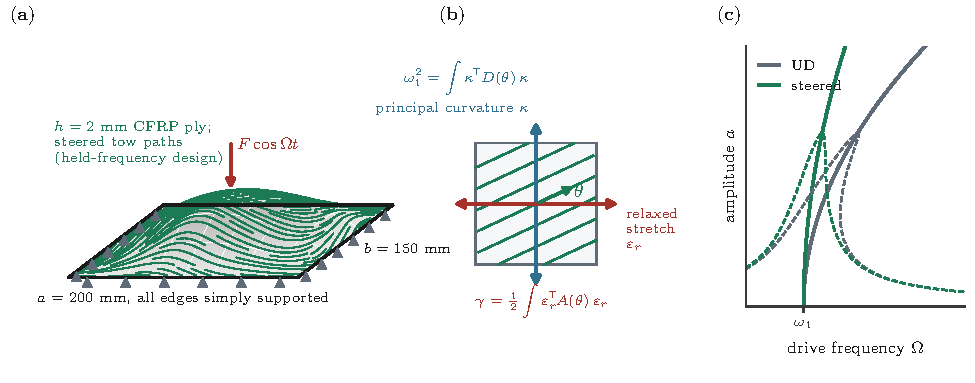
\includegraphics[width=\linewidth]{figs/fig_schematic.pdf}
\caption{The problem and the hypothesis. \textbf{(a)}~A simply supported
$200\times150\times2$\,mm CFRP plate, drawn deflected in its fundamental mode, with the tow
paths of the held-frequency steered design of Sec.~\ref{sec:levers} and the harmonic center
load. \textbf{(b)}~What one material point sees: the fiber direction $\theta$, the principal
curvature of the mode, which with the bending stiffness $\bm D(\theta)$ sets $\omega_1^2$, and
the principal relaxed stretch (drawn at the plate's typical $33^\circ$ conflict with the
curvature, Sec.~\ref{sec:mechanism}), which with the membrane stiffness $\bm A(\theta)$ sets
the hardening $\gamma$ (Sec.~\ref{sec:model}). \textbf{(c)}~The consequence, sketched: at the
same linear frequency $\omega_1$, a smaller hardening bends the backbone (solid) less, and the
forced response (dashed) of the unidirectional plate folds and jumps where the steered one
stays single-valued (Sec.~\ref{sec:jumpres}).}
\label{fig:schematic}
\end{figure}

\paragraph{Hypothesis.} (Fig.~\ref{fig:schematic}.) The linear frequency and the hardening
are integrals of the \emph{same} rotated stiffness tensor against two \emph{different}
strain fields of the fundamental mode. The frequency is set by the bending curvature,
$\omega_1^2=\int\bm\kappa^{\!\top}\bm D(\theta)\bm\kappa$. The hardening is set by the
membrane stretch the mode induces after the in-plane field has relaxed,
$\gamma=\tfrac12\int\bm\varepsilon_r^{\!\top}\bm A(\theta)\bm\varepsilon_r$
(Sec.~\ref{sec:model}). The two strain fields differ from point to point in magnitude
and in principal direction. We hypothesize that a spatially varying fiber angle can
therefore satisfy, \emph{pointwise}, a trade-off between the two energies that a uniform
angle can only satisfy \emph{on average}. Where stretching energy dominates, the fibers turn
across the principal stretch. Where bending energy dominates, they are set toward or away
from the principal curvature as the frequency constraint requires (away from it when the
frequency is held at the UD value, the lowest of all uniform layups). Stacking separates the
same two functionals in the classical way, through the thickness ($\bm D$ weights the outer
plies, $\bm A$ all plies equally \cite{tsai1968}); it is the competing freedom against which
the in-plane route is tested. Section~\ref{sec:theory} turns the hypothesis into precise
statements, which make five falsifiable predictions:
\begin{enumerate}[label=\textbf{P\arabic*},leftmargin=2.2em,itemsep=1pt]
\item An isotropic material offers no orientation lever at all
  (Corollary~\ref{cor:iso}).
\item For a single-ply beam, any uniform angle leaves the frequency-normalized hardening
  \emph{exactly} unchanged, so every gain must come from spatial variation. The
  optimal variation places compliant fibers where the mode does not bend: the inflection
  points (Proposition~\ref{prop:beam}).
\item On a plate, a steered field reaches combinations of linear frequency and hardening
  that no uniform layup reaches, whether a single angle or a stacking sequence.
\item The optimized orientation follows the local preferred directions of the two
  energies. A first-order pointwise design computed from the unidirectional mode alone
  already captures most of the gain (Proposition~\ref{prop:pointwise}).
\item The lever grows with the material anisotropy and with the conflict between the two
  strain fields, and is limited by the tow-curvature constraint relative to the length scale
  of those fields.
\end{enumerate}
\noindent A consequence follows if the predictions hold. The jump-free amplitude scales
as $J^{-1/2}$ (Proposition~\ref{prop:cusp}), so reducing the hardening at held frequency
widens the panel's hysteresis-free operating range by a predictable factor. That factor is a
property of the conservative backbone; the absolute thresholds also depend on damping and
forcing.

\subsection{Approach}
We test the predictions on a clamped laminated beam and on simply supported and clamped
laminated plates, all von K\'arm\'an. The backbone is computed by an SSM reduction verified
against analytic, harmonic-balance (EPMC) and finite-element references. For design we use
the SSM's hardening coefficient in a closed form that is exact for the in-plane relaxation
and evaluated on a \emph{mode-adaptive} fundamental, with an analytic adjoint. The plate
frequency is an equality constraint and the beam frequency a floor
($\omega_1\geq0.98\,\omega_{1,\UD}$). The tow-curvature limit is imposed pointwise. The
held-frequency plate design is then checked on refined bases, on an independent
finite-element model with the frequency re-matched, on the full multi-mode model (by its
SSM, by EPMC continuation and by time integration of up/down frequency sweeps), for other
supports, aspect ratios, damping laws and edge restraints, and under an as-built tow-defect
model.

\begin{center}
\fbox{\begin{minipage}{0.94\linewidth}\small
\textbf{What ``exact'' means in this paper.} Three levels are kept apart.
\emph{(i) Exact statements} are proved for the stated model class: the Fourier structure
(Proposition~\ref{prop:fourier}), isotropic annihilation (Corollary~\ref{cor:iso}), beam
invariance (Corollary~\ref{cor:beaminv}) and the UD floor among uniform laminates
(Corollary~\ref{cor:udfloor}). \emph{(ii) Exact within the discretized design model}: the
in-plane relaxation is exact for the adopted von K\'arm\'an kinematics and in-plane basis
(Proposition~\ref{prop:relaxed}), and the frequency equality holds to $10^{-10}$ on the design
basis. \emph{(iii) Approximate across models}: on finer bases and an independent finite-element
model, the steered frequency differs from the UD value by up to $\nHeldTol\%$. We therefore also
report the hardening ratio with the frequency re-matched in each of those models
(Sec.~\ref{sec:confirm}). The cubic backbone itself is a small-amplitude approximation, valid
over the amplitude range verified against full-order EPMC (Appendix~\ref{app:calib}).
\end{minipage}}
\end{center}

\paragraph{Organization.} Section~\ref{sec:model} states the model, the reduction and the
backbone and jump quantities. Section~\ref{sec:theory} develops the mechanism and its
predictions. Section~\ref{sec:design} poses the design problem and derives its
sensitivities. Section~\ref{sec:results} tests P1--P5, the robustness of the result and the
consequence for the forced response. Section~\ref{sec:discussion} states what the results do
and do not establish. The appendices give the SSM recursion, the SSM--condensation
equivalence, the finite-element validation, calibration against prior work, and a
verification and reproducibility map.

\section{Model, reduction, and the quantities we design}\label{sec:model}

\subsection{Laminate constitutive model}\label{sec:clt}
A unidirectional CFRP lamina ($E_1=\SI{131}{GPa}$, $E_2=\SI{9}{GPa}$,
$G_{12}=\SI{5}{GPa}$, $\nu_{12}=0.27$, $\rho=\SI{1600}{kg/m^3}$) has the on-axis
plane-stress stiffness $\bm Q$, with $Q_{11}=E_1/(1-\nu_{12}\nu_{21})$,
$Q_{22}=E_2/(1-\nu_{12}\nu_{21})$, $Q_{12}=\nu_{12}Q_{22}$, $Q_{66}=G_{12}$ and
$\nu_{21}=\nu_{12}E_2/E_1$. In engineering Voigt notation (strain
$\bm s=[s_{xx},s_{yy},2s_{xy}]^{\!\top}$), rotating the fibers through $\theta$ gives
\begin{equation}
\bar{\bm Q}(\theta)=\bm T(\theta)\,\bm Q\,\bm T(\theta)^{\!\top},\qquad
\bm T(\theta)=\begin{bmatrix}c^2&s^2&-2sc\\ s^2&c^2&2sc\\ sc&-sc&c^2-s^2\end{bmatrix},
\quad (c,s)=(\cos\theta,\sin\theta).
\label{eq:rot}
\end{equation}
Its entries are trigonometric polynomials of degree four in $\theta$ (Tsai--Pagano \cite{tsai1968}):
\begin{equation}
\bar{\bm Q}(\theta)=\bm\Gamma_0+\cos2\theta\,\bm\Gamma_1+\sin2\theta\,\bm\Gamma_2
+\cos4\theta\,\bm\Gamma_3+\sin4\theta\,\bm\Gamma_4,
\label{eq:qbar}
\end{equation}
\begin{gather*}
\bm\Gamma_0=\begin{bmatrix}U_1&U_4&0\\U_4&U_1&0\\0&0&U_5\end{bmatrix},\quad
\bm\Gamma_1=\begin{bmatrix}U_2&0&0\\0&-U_2&0\\0&0&0\end{bmatrix},\quad
\bm\Gamma_2=\tfrac{U_2}{2}\begin{bmatrix}0&0&1\\0&0&1\\1&1&0\end{bmatrix},\\
\bm\Gamma_3=U_3\begin{bmatrix}1&-1&0\\-1&1&0\\0&0&-1\end{bmatrix},\quad
\bm\Gamma_4=U_3\begin{bmatrix}0&0&1\\0&0&-1\\1&-1&0\end{bmatrix},
\end{gather*}
with the material invariants
$U_1=\tfrac18(3Q_{11}+3Q_{22}+2Q_{12}+4Q_{66})$, $U_2=\tfrac12(Q_{11}-Q_{22})$,
$U_3=\tfrac18(Q_{11}+Q_{22}-2Q_{12}-4Q_{66})$, $U_4=\tfrac18(Q_{11}+Q_{22}+6Q_{12}-4Q_{66})$,
$U_5=\tfrac18(Q_{11}+Q_{22}-2Q_{12}+4Q_{66})$. $\bm\Gamma_0$ is isotropic. All the
dependence on orientation is carried by $U_2$ and $U_3$, which vanish for an isotropic
material. For the CFRP above, $U_2/U_1=1.10$ and $U_3/U_1=0.26$.

A symmetric laminate ($\bm B=\bm 0$) of thickness $h$ has the membrane and bending
stiffnesses
\begin{equation}
\bm A=h\Big[\bm\Gamma_0+\textstyle\sum_{i=1}^4\xi^A_i\bm\Gamma_i\Big],\qquad
\bm D=\tfrac{h^3}{12}\Big[\bm\Gamma_0+\textstyle\sum_{i=1}^4\xi^D_i\bm\Gamma_i\Big],
\label{eq:lampar}
\end{equation}
with the lamination parameters \cite{tsai1968,abdalla2007}
\begin{equation}
\bm\xi^A=\int_{-1/2}^{1/2}\bm v(\theta(\bar z))\,\dd\bar z,\qquad
\bm\xi^D=12\int_{-1/2}^{1/2}\bar z^2\,\bm v(\theta(\bar z))\,\dd\bar z,\qquad
\bm v(\theta)=(\cos2\theta,\sin2\theta,\cos4\theta,\sin4\theta),
\label{eq:xi}
\end{equation}
where $\theta(\bar z)$ is the ply angle at normalized height $\bar z=z/h$. Two facts
organize everything that follows.
\begin{itemize}[itemsep=1pt]
\item A \emph{single-ply-like} laminate (one angle through the thickness) has
$\bm\xi^A=\bm\xi^D=\bm v(\theta)$, so $\bm D=\tfrac{h^2}{12}\bm A$ pointwise.
\item A \emph{stacking sequence} makes $\bm\xi^D\ne\bm\xi^A$. Because $\bm\xi^D$ weights
the outer plies by $12\bar z^2$, the stacking sequence separates bending from membrane
stiffness \emph{through the thickness}.
\end{itemize}
A \emph{steered} laminate makes $\bm\xi^{A,D}$ functions of the in-plane position
$\bm x$.

\subsection{The laminated von K\'arm\'an plate}\label{sec:plate}
A rectangular plate $\Omega=[0,a]\times[0,b]$ ($a=\SI{0.20}{m}$, $b=\SI{0.15}{m}$,
$h=\SI{2}{mm}$) carries the transverse deflection $w$ and in-plane displacements
$\bm u=(u,v)$. The von K\'arm\'an membrane strain and curvature are
\begin{equation}
\bm\varepsilon=\bm\varepsilon_L(\bm u)+\bm\varepsilon_{NL}(w),\quad
\bm\varepsilon_L=\begin{bmatrix}u_{,x}\\v_{,y}\\u_{,y}+v_{,x}\end{bmatrix},\quad
\bm\varepsilon_{NL}=\tfrac12\begin{bmatrix}w_{,x}^2\\w_{,y}^2\\2w_{,x}w_{,y}\end{bmatrix},\qquad
\bm\kappa=-\begin{bmatrix}w_{,xx}\\w_{,yy}\\2w_{,xy}\end{bmatrix},
\label{eq:kin}
\end{equation}
and, with $\bm A(\bm x),\bm D(\bm x)$ from \eqref{eq:lampar}, the strain energy is
\begin{equation}
U=\tfrac12\!\int_\Omega\!\bm\kappa^{\!\top}\bm D\,\bm\kappa\,\dd\Omega
+\tfrac12\!\int_\Omega\!(\bm\varepsilon_L+\bm\varepsilon_{NL})^{\!\top}\bm A\,
(\bm\varepsilon_L+\bm\varepsilon_{NL})\,\dd\Omega .
\label{eq:energy}
\end{equation}
With the kinetic energy $T=\tfrac12\int\rho h(\dot w^2+|\dot{\bm u}|^2)$, Hamilton's
principle gives the laminated F\"oppl--von K\'arm\'an equations \cite{amabili2008},
\begin{equation}
N_{\alpha\beta,\beta}=\rho h\,\ddot u_\alpha,\qquad
M_{\alpha\beta,\alpha\beta}+\big(N_{\alpha\beta}w_{,\beta}\big)_{,\alpha}+p=\rho h\,\ddot w,
\qquad \bm N=\bm A(\bm\varepsilon_L+\bm\varepsilon_{NL}),\ \bm M=\bm D\bm\kappa .
\label{eq:fvk}
\end{equation}
The edges are simply supported and immovable ($w=0$, $\bm u=\bm 0$ on $\partial\Omega$).
We discretize by Galerkin's method on sine bases, which satisfy these conditions term by
term:
\begin{equation}
w=\sum_{k=1}^{N_w}q_k\,\phi_k,\quad \phi_k=\sin\tfrac{m_k\pi x}{a}\sin\tfrac{n_k\pi y}{b};
\qquad
u,v=\sum_{j=1}^{N_s}s^{u,v}_j\,\psi_j,\quad \psi_j=\sin\tfrac{i_j\pi x}{a}\sin\tfrac{l_j\pi y}{b}.
\end{equation}
We use $N_w=64$ ($m,n\le8$) and $N_s=36$ per component. For the robustness study of
Sec.~\ref{sec:robust} the same evaluator is built on two other bases: clamped edges
($w=\partial_nw=0$) with $\phi_k=\sin\tfrac{\pi x}{a}\sin\tfrac{m_k\pi x}{a}\,
\sin\tfrac{\pi y}{b}\sin\tfrac{n_k\pi y}{b}$, which reproduces the clamped isotropic square
plate's frequency parameter $35.99$ to $0.15\%$; and in-plane traction-free (``movable'') edges,
with a Chebyshev polynomial basis of degree $\le10$ for $u,v$, converged to four digits in
$\gamma$. The bases are converged
for the steered designs: Table~\ref{tab:conv} shows that the steered relaxation needs at least
five to six in-plane modes per direction; the three-mode basis that suffices for a uniform
laminate under-resolves it badly ($J/J_{\UD}=\nConvThree$ instead of $\nConvBase$).

\begin{table}[!tbp]
\centering\footnotesize
\caption{Convergence of the evaluator on the reported held-frequency steered design
(generated by \texttt{conv\_table.py}). $J/J_{\UD}$ and the relaxed share are converged on
the bold basis; three in-plane modes per direction under-resolve the steered relaxation.
The steered frequency is a Ritz upper bound that falls by $\nConvFreqDrop\%$ as the transverse basis
grows (the UD frequency does not change), so ``held frequency'' holds to about $\nConvFreqDrop\%$
across bases and $\nHeldTol\%$ against the independent FE model.
Bold: the basis used throughout.}
\label{tab:conv}
\IfFileExists{conv_table.tex}{\begin{tabular}{@{}ccccccc@{}}
\toprule
transverse $m,n\le$ & in-plane $i,j\le$ & $f_{1,\UD}$ (Hz) & $f_1$ (Hz) & $J/J_{\UD}$ & relaxed share (UD) & relaxed share (steered)\\ \midrule
8 & 3 & 256.3 & 256.3 & 0.523 & 33\% & 31\%\\
8 & 4 & 256.3 & 256.3 & 0.420 & 33\% & 44\%\\
8 & 5 & 256.3 & 256.3 & 0.375 & 33\% & 50\%\\
\bf 8 & \bf 6 & \bf 256.3 & \bf 256.3 & \bf 0.366 & \bf 33\% & \bf 51\%\\
8 & 8 & 256.3 & 256.3 & 0.360 & 33\% & 52\%\\
12 & 6 & 256.3 & 254.6 & 0.370 & 33\% & 51\%\\
12 & 8 & 256.3 & 254.6 & 0.364 & 33\% & 52\%\\
16 & 8 & 256.3 & 253.9 & 0.366 & 33\% & 51\%\\
\bottomrule
\end{tabular}
}{\textit{table pending}}
\end{table}

With $\bm x=[\bm q;\bm s]$ the system is
\begin{equation}
\bm M\ddot{\bm x}+\bm C\dot{\bm x}+\bm K\bm x+\bm B_2(\bm x,\bm x)+\bm T_3(\bm x,\bm x,\bm x)=\bm f(t),
\label{eq:eom}
\end{equation}
with
$M_{kl}=\rho h\int\phi_k\phi_l$ (likewise for $\psi$),
$\bm K=\mathrm{blkdiag}(\bm K_b,\bm K_{\mathrm{in}})$,
$(\bm K_b)_{kl}=\int\bm\kappa_k^{\!\top}\bm D\bm\kappa_l$ and
$(\bm K_{\mathrm{in}})_{jl}=\int\bm\varepsilon_{L,j}^{\!\top}\bm A\bm\varepsilon_{L,l}$.
$\bm B_2$ is the gradient of $\int\bm\varepsilon_L^{\!\top}\bm A\bm\varepsilon_{NL}$ (the
$\bm u\leftrightarrow w^2$ coupling) and $\bm T_3$ is the gradient of
$\tfrac12\int\bm\varepsilon_{NL}^{\!\top}\bm A\bm\varepsilon_{NL}$ (the membrane cubic).
Because $\bm B=\bm 0$, the \emph{linear} problem decouples into a bending block and an
in-plane block. The mass is design-independent: every design in this paper has the
same plate, the same material and the same thickness.

The \emph{beam} is the one-dimensional specialization: a clamped--clamped strip
($L=\SI{0.30}{m}$, width $\SI{20}{mm}$, $h=\SI{2}{mm}$) with axial $u$ and transverse
$w$, $\varepsilon=u'+\tfrac12w'^2$ and $\kappa=-w''$. For a single-ply laminate,
$A=bhE(x)$ and $D=\tfrac{bh^3}{12}E(x)$ with $E(x)=\bar Q_{11}(\theta(x))$. It is
discretized by Hermite-cubic/linear elements, and the axial ends are immovable.

\subsection{Spectral submanifold and backbone}\label{sec:ssm}
In first-order form $\bm z=[\bm x;\dot{\bm x}]$,
$\bm{\mathcal B}\dot{\bm z}=\bm{\mathcal A}\bm z+\bm F(\bm z)$ with
$\bm{\mathcal B}=\begin{bsmallmatrix}\bm C&\bm M\\\bm M&\bm0\end{bsmallmatrix}$,
$\bm{\mathcal A}=\begin{bsmallmatrix}-\bm K&\bm0\\\bm0&\bm M\end{bsmallmatrix}$ and
$\bm F=[-\bm B_2-\bm T_3;\bm0]$. Let $\lambda_1,\bar\lambda_1$ be the eigenvalues of the
fundamental, with right eigenvector $\bm v_1$ and left eigenvector $\bm u_1$
($\bm u_1^*\bm{\mathcal A}=\lambda_1\bm u_1^*\bm{\mathcal B}$,
$\bm u_1^*\bm{\mathcal B}\bm v_1=1$). The SSM $\mathcal W$ is the unique smoothest
invariant manifold tangent to their eigenspace \cite{haller2016}. It exists if
$\lambda_1$ is the slowest pair and no outer eigenvalue equals
$m_1\lambda_1+m_2\bar\lambda_1$ up to the truncation order. Parametrizing
$\bm z=\bm W(\bm p)$ and $\dot{\bm p}=\bm R(\bm p)$ gives the invariance equation
$\bm{\mathcal B}\,\mathrm D\bm W\,\bm R=\bm{\mathcal A}\bm W+\bm F(\bm W)$. Expanding both
maps in monomials $\bm p^{\bm m}$, it separates order by order into the homological
equations
\begin{equation}
(\Lambda_{\bm m}\bm{\mathcal B}-\bm{\mathcal A})\bm w_{\bm m}
+\bm{\mathcal B}(\bm v_1R^1_{\bm m}+\bar{\bm v}_1R^2_{\bm m})=\bm G_{\bm m},
\qquad \Lambda_{\bm m}=m_1\lambda_1+m_2\bar\lambda_1,
\label{eq:homological}
\end{equation}
where $\bm G_{\bm m}$ collects lower-order terms (Appendix~\ref{app:coeffs}). At the
near-resonant indices $\bm m=(k{+}1,k)$ the operator is (near-)singular. Projecting onto
$\bm u_1$ gives the reduced (normal-form) coefficients
$\gamma_{2k+1}=\bm u_1^*\bm G_{(k+1,k)}$. On the orbit
$p_1=\tfrac\rho2e^{i\vartheta}$, $p_2=\bar p_1$, the backbone and the modal decay rate are
\begin{equation}
\Om(\rho)=\Imag\Big(\lambda_1+\sum_{k\ge1}\gamma_{2k+1}\big(\tfrac{\rho}{2}\big)^{2k}\Big),\qquad
\alpha(\rho)=\Real(\cdots).
\label{eq:backbone}
\end{equation}
The implementation is verified against the analytic Duffing backbone through fifth
order ($3/8$ and $-21/256$), against full-order EPMC continuation, and against two
published results \cite{pozzi2025} (Appendix~\ref{app:calib}). The master
eigenvector is computed by Rayleigh-quotient inverse iteration on the complex-symmetric
pencil, with $\bm u_1=\bar{\bm v}_1$. A dense QZ solve of the stiff first-order pencil was
found to lose up to ten digits (eigenvector condition number $\sim10^{14}$ for laminated
beams) and is no longer used for symmetric systems (regression test in
\texttt{tests/test\_relaxed\_plate.py}).

\subsection{The relaxed hardening coefficient}\label{sec:relaxed}
Let the fundamental be the lowest Ritz pair of the bending block,
$\bm K_b\bm v=\omega_1^2\bm M_w\bm v$ with $\bm v^{\!\top}\bm M_w\bm v=1$. Its shape
$w_1=\sum_kv_k\phi_k$ \emph{adapts} to the stiffness field. This is the exact linear
master mode of \eqref{eq:eom}, because the blocks decouple when $\bm B=\bm0$. Write its
curvature as $\bm\kappa_1$ and its stretch as
\begin{equation}
\bm m=\big[w_{1,x}^2,\;w_{1,y}^2,\;2w_{1,x}w_{1,y}\big]^{\!\top}=2\bm\varepsilon_{NL}(w_1).
\end{equation}

\begin{proposition}[Relaxed cubic, variational form]\label{prop:relaxed}
Let the in-plane field be slaved quasi-statically to $q^2$, the square of the
fundamental's modal amplitude. Then the cubic coefficient of the single-mode reduced
dynamics $\ddot q+\omega_1^2q+\gamma q^3=0$ is
\begin{equation}
\gamma=\min_{\bm s}\;\tfrac12\int_\Omega(\bm m-2\bm\varepsilon_L(\bm s))^{\!\top}\bm A\,
(\bm m-2\bm\varepsilon_L(\bm s))\,\dd\Omega
=k_{nl}-2\,\bm g^{\!\top}\bm K_{\mathrm{in}}^{-1}\bm g
=\tfrac12\int_\Omega\bm\varepsilon_r^{\!\top}\bm A\,\bm\varepsilon_r\,\dd\Omega,
\label{eq:gamma}
\end{equation}
with $k_{nl}=\tfrac12\int\bm m^{\!\top}\bm A\bm m$,
$\bm g=\tfrac12\int\bm\varepsilon_L(\cdot)^{\!\top}\bm A\bm m$,
$\bm s^\star=\bm K_{\mathrm{in}}^{-1}\bm g$ and the relaxed stretch
$\bm\varepsilon_r=\bm m-2\bm\varepsilon_L(\bm s^\star)$.
\end{proposition}
\begin{proof}
With $w=qw_1$ and $\bm u=-q^2\bm s$, the membrane strain is
$\bm\varepsilon=\tfrac{q^2}{2}(\bm m-2\bm\varepsilon_L(\bm s))$. The membrane energy is
therefore $\tfrac{q^4}{8}\int(\bm m-2\bm\varepsilon_L(\bm s))^{\!\top}\bm A(\cdot)
=\tfrac{q^4}{4}F(\bm s)$, where $F(\bm s)=k_{nl}-4\bm s^{\!\top}\bm g+2\bm s^{\!\top}
\bm K_{\mathrm{in}}\bm s$. Static equilibrium of the in-plane field minimizes $F$, at
$\bm s^\star=\bm K_{\mathrm{in}}^{-1}\bm g$, with $F(\bm s^\star)=k_{nl}-2\bm g^{\!\top}
\bm K_{\mathrm{in}}^{-1}\bm g$. The reduced potential $\tfrac{\gamma}{4}q^4$ then gives
\eqref{eq:gamma}. The last form is $F(\bm s^\star)$ written out.
\end{proof}

Proposition~\ref{prop:relaxed} has three uses. (i) $k_{nl}$ is the restrained
(immovable in-plane field) upper bound, and $2\bm g^{\!\top}\bm K_{\mathrm{in}}^{-1}\bm g$
is the \emph{relaxation}. Its share of $k_{nl}$ is $\nRelaxUD\%$ for the unidirectional
plate. (ii) Because $\gamma$ is a \emph{minimum} over $\bm s$, its design derivative
needs no in-plane adjoint (envelope theorem; Sec.~\ref{sec:sens}). (iii) It writes the
hardening as the integral of an energy density (Sec.~\ref{sec:theory}).

\begin{proposition}[Agreement with the SSM]\label{prop:ssmcond}
For an undamped system \eqref{eq:eom} with $\bm B=\bm 0$, the cubic SSM coefficient of the
fundamental satisfies
$\Imag\gamma_3=\tfrac{3}{2\omega_1}\gamma\,[1+O(4\omega_1^2/\omega_{\mathrm{in}}^2)]$,
where $\omega_{\mathrm{in}}$ is the lowest in-plane frequency.
\end{proposition}
\noindent The proof is in Appendix~\ref{app:ssmcond}. In short: the $(1,1)$ in-plane
homological solve is exactly static ($\Lambda_{(1,1)}=0$), and the $(2,0)$ solve is
static up to the resolvent factor
$(\bm K_{\mathrm{in}}-4\omega_1^2\bm M_{\mathrm{in}})^{-1}$. For our plate
$4\omega_1^2/\omega_{\mathrm{in}}^2=\nRhoIn$ ($f_{\mathrm{in}}\approx\nFin$\,kHz on the full multi-mode plate), and \eqref{eq:gamma} reproduces the full
multi-mode SSM coefficient to within $\nSSMvsEval\%$ (Sec.~\ref{sec:confirm}).

\subsection{The backbone in physical amplitude, and the design quantity $J$}
For $\ddot q+\omega_1^2q+\gamma q^3=0$ the cubic SSM gives
$\Om=\omega_1+\tfrac38(\gamma/\omega_1)q^2$. The mid-plate deflection of the mode is
$a=w_cq$, with $w_c=w_1(a/2,b/2)$, so
\begin{equation}
\frac{\Om}{\omega_1}=1+\frac38J\,a^2=1+\beta\Big(\frac{a}{h}\Big)^2,\qquad
J=\frac{\gamma}{\omega_1^2w_c^2},\qquad \beta=\tfrac38Jh^2 .
\label{eq:J}
\end{equation}
$J$ (units m$^{-2}$) is the \emph{frequency-normalized detuning}. It is invariant to the
mode normalization, and it is what we design. The unidirectional plate has
$f_1=\nUDf$\,Hz, $\beta=\nEvBetaUD$ and a $\nUDdet\%$ shift at $a/h=0.4$.
The cubic truncation reproduces the full-order EPMC detuning to within $\nEPMCAgree\%$ over the
amplitudes EPMC reached, $a/h\le\nEPMCmaxUD$ (UD) and $\le\nEPMCmaxOpt$ (steered) (Appendix~\ref{app:calib}).

\subsection{Forced response and the jump-free amplitude}\label{sec:jumpth}
With harmonic forcing $\bm f\cos\Om t$ and damping $\bm C=2\zeta\omega_1\bm M$, seeking
$p_1=\tfrac\rho2e^{i\Om t}$ on the SSM gives the leading-order forced-response curve
\begin{equation}
\big[(\Om-\Om(\rho))^2+\alpha(\rho)^2\big]\rho^2=|f_1|^2,\qquad f_1=\bm u_1^*[\bm f;\bm0].
\label{eq:frc}
\end{equation}

\begin{proposition}[Jump-free amplitude]\label{prop:cusp}
For the cubic backbone \eqref{eq:J} with $\alpha=\zeta\omega_1$, the forced response
\eqref{eq:frc} is single-valued in $\Om$ for every drive whose peak (resonant) amplitude is
below
\begin{equation}
\frac{a_c}{h}=\Big(\frac{8\zeta}{3\sqrt3\,\beta}\Big)^{1/2}\;\propto\;J^{-1/2},
\label{eq:ac}
\end{equation}
and multivalued (a fold pair with jump and hysteresis) above it. At the critical drive the
vertical tangent sits at the lower amplitude $(\sqrt3/2)\,a_c$ on the response curve.
\end{proposition}
\begin{proof}
Write $x=a^2$, $c=\omega_1\beta/h^2$, $\mu=\zeta\omega_1$, and let $F$ be the drive
expressed in physical amplitude. Then \eqref{eq:frc} reads
$[(\sigma-cx)^2+\mu^2]x=F^2$, with $\sigma=\Om-\omega_1$. Put $\sigma=cx+s$. The curve is
$x=F^2/(s^2+\mu^2)$, $\sigma=cF^2/(s^2+\mu^2)+s$, and it folds where $\dd\sigma/\dd s=0$,
i.e.\ where $2cF^2s=(s^2+\mu^2)^2$. A fold pair first appears when this equation has a
double root, i.e.\ when $2cF^2=4s(s^2+\mu^2)$ also holds. Combining the two conditions
gives $s^2+\mu^2=4s^2$, so $s=\mu/\sqrt3$, and the critical drive is
$F_c^2=(s^2+\mu^2)^2/(2cs)=8\mu^3/(3\sqrt3\,c)$. The vertical tangent lies at
$x=F_c^2/(s^2+\mu^2)=2\mu/(\sqrt3c)$, while the peak of the response (at $s=0$) is
$x_c=F_c^2/\mu^2=8\mu/(3\sqrt3\,c)$, which is \eqref{eq:ac}. Below $F_c$ the curve has no
fold; above it, it has two.
\end{proof}
\noindent Proposition~\ref{prop:cusp} is the consequence we test. Holding $\omega_1$,
$\zeta$ and $h$ and reducing $J$ by a factor $r$ widens the jump-free amplitude by
$r^{-1/2}$. In Sec.~\ref{sec:confirm} we compute $a_c$ \emph{numerically}, as the drive
at which the full-order damped SSM response first becomes multivalued, and compare it
with \eqref{eq:ac}.

\section{Theory: why a fiber field can decouple hardening from frequency}\label{sec:theory}

\subsection{Two energy densities over one stiffness}
With the mass-normalized adapted mode, the Rayleigh quotient and
Proposition~\ref{prop:relaxed} write both design quantities as integrals of local energy
densities:
\begin{equation}
\omega_1^2=\int_\Omega e_K\,\dd\Omega,\quad e_K=\bm\kappa_1^{\!\top}\bm D\,\bm\kappa_1;\qquad
\gamma=\int_\Omega e_G\,\dd\Omega,\quad e_G=\tfrac12\bm\varepsilon_r^{\!\top}\bm A\,\bm\varepsilon_r .
\label{eq:densities}
\end{equation}
$J=\gamma/(\omega_1^2w_c^2)$ is their ratio up to the mode's mid-plate value. Both
densities read the \emph{same} rotated material \eqref{eq:qbar}, but through different
strain fields: $\bm\kappa_1$ (second derivatives of $w_1$, largest where the mode bends)
and $\bm\varepsilon_r$ (squared first derivatives minus the in-plane relief). For the simply
supported fundamental both peak at the center, but with different principal directions
(Sec.~\ref{sec:mechanism}). The following proposition shows exactly how
each density depends on the local fiber angle.

\subsection{Local Fourier structure}
\begin{proposition}[Angular dependence of a laminate energy density]\label{prop:fourier}
Let $\bm s$ be an engineering strain vector whose tensor has principal values
$e_{\max},e_{\min}$, ordered so that $|e_{\max}|\ge|e_{\min}|$, and let $\hat\varphi$ be the
direction of $e_{\max}$. Then for the single-ply stiffness \eqref{eq:qbar},
\begin{equation}
\bm s^{\!\top}\bar{\bm Q}(\theta)\bm s=
\underbrace{U_1(e_{\max}^2+e_{\min}^2)+2U_4e_{\max}e_{\min}}_{\text{isotropic}}
+U_2\,\Delta\cos2(\theta-\hat\varphi)+U_3\,\Sigma\cos4(\theta-\hat\varphi),
\label{eq:fourier}
\end{equation}
with $\Delta=e_{\max}^2-e_{\min}^2\ge0$ and $\Sigma=(e_{\max}-e_{\min})^2\ge0$.
\end{proposition}
\begin{proof}
Rotation invariance gives $\bm s^{\!\top}\bar{\bm Q}(\theta)\bm s=\bm s'^{\!\top}\bar{\bm
Q}(\theta-\hat\varphi)\bm s'$, with $\bm s'=[e_{\max},e_{\min},0]^{\!\top}$ the strain in
its principal frame. Let $\psi=\theta-\hat\varphi$. Using \eqref{eq:qbar},
$\bar Q_{11}=U_1+U_2\cos2\psi+U_3\cos4\psi$,
$\bar Q_{22}=U_1-U_2\cos2\psi+U_3\cos4\psi$ and $\bar Q_{12}=U_4-U_3\cos4\psi$, we get
$\bar Q_{11}e_{\max}^2+2\bar Q_{12}e_{\max}e_{\min}+\bar Q_{22}e_{\min}^2
=U_1(e_{\max}^2+e_{\min}^2)+2U_4e_{\max}e_{\min}+U_2(e_{\max}^2-e_{\min}^2)\cos2\psi
+U_3(e_{\max}-e_{\min})^2\cos4\psi$.
\end{proof}

Applying \eqref{eq:fourier} to the two densities, pointwise:
\begin{align}
e_K(\bm x,\theta)&=\tfrac{h^3}{12}\big[I_K+U_2\Delta_K\cos2(\theta-\varphi_K)+U_3\Sigma_K\cos4(\theta-\varphi_K)\big],
\label{eq:eK}\\
e_G(\bm x,\theta)&=\tfrac{h}{2}\big[I_G+U_2\Delta_G\cos2(\theta-\varphi_G)+U_3\Sigma_G\cos4(\theta-\varphi_G)\big],
\label{eq:eG}
\end{align}
where $(\Delta_K,\Sigma_K,\varphi_K)$ come from the principal curvatures of $w_1$ and
$(\Delta_G,\Sigma_G,\varphi_G)$ from the principal relaxed stretches. For CFRP
$U_2\approx\nUtwoUthree\,U_3$, so the $2\theta$ harmonic dominates. To leading order, then:
\begin{itemize}[itemsep=1pt]
\item $e_K$ is largest (the point contributes most to $\omega_1^2$) when the fiber lies
\emph{along} the principal curvature, $\theta=\varphi_K$;
\item $e_G$ is smallest (the point contributes least to $\gamma$) when the fiber lies
\emph{across} the principal stretch, $\theta=\varphi_G+\pi/2$.
\end{itemize}
Which way the frequency pulls depends on the sign of the multiplier $\Lambda$ of
Proposition~\ref{prop:pointwise} below, which weights $e_K$ against $e_G$. If the target
frequency lies above the one the stretch alone would select, $\Lambda>0$ and the fiber is
drawn toward the principal curvature, $\theta=\varphi_K$. If it lies below, $\Lambda<0$
and the fiber is pushed \emph{across} the principal curvature, $\theta=\varphi_K+\pi/2$,
the bending-compliant direction. We call $\varphi_G+\pi/2$ and the frequency-favored
direction the \emph{preferred directions}, and the angle between them,
$\chi(\bm x)\in[0,\pi/2]$, the \emph{conflict}. Where $\chi=0$, one fiber direction
serves both energies. Where $\chi$ is large, any single direction compromises.

\begin{corollary}[The unidirectional floor]\label{cor:udfloor}
Among all uniform symmetric laminates of the same thickness and mass, whatever the
stacking sequence, the lowest linear frequency is attained by a single-angle laminate.
\end{corollary}
\begin{proof}
For a symmetric laminate $\bm D=\tfrac{h^3}{12}\big(\bm\Gamma_0+\sum_k\xi^D_k\bm\Gamma_k\big)$ is affine
in its four lamination parameters $\bm\xi^D$, and the set of $\bm\xi^D$ reachable by
stacking lies in the convex hull of the single-angle curve
$\bm\xi^D(\theta)=(\cos2\theta,\sin2\theta,\cos4\theta,\sin4\theta)$ \cite{tsai1968}.
$\omega_1^2$ is the minimum over admissible $w$ of a Rayleigh quotient that is affine in
$\bm\xi^D$, hence a concave function of $\bm\xi^D$, and a concave function on a convex
hull attains its minimum at an extreme point, i.e.\ at a single-angle laminate.
\end{proof}
\noindent For the plate studied here the single-angle frequency rises monotonically from
$\theta=0^\circ$ (Sec.~\ref{sec:levers}), so UD is the lowest-frequency uniform laminate of
\emph{any} stacking sequence, not only of the enumerated ones, and at $\omega_{1,\UD}$ there
is no other uniform competitor.

\begin{corollary}[P1: isotropy annihilates the lever]\label{cor:iso}
If $U_2=U_3=0$, then $\bm A$ and $\bm D$ are independent of every ply angle at every point.
Hence $\omega_1$, $\gamma$ and $J$ are independent of the orientation field, uniform or
steered or stacked, and every orientation sensitivity vanishes identically. This is exact,
including mode adaptation and relaxation, because the operators themselves do not depend
on $\theta$.
\end{corollary}
\noindent Numerically, $\partial J/\partial\theta\equiv0$ to $10^{-10}$ relative when
$\bm Q$ is set isotropic (\texttt{tests/test\_relaxed\_plate.py}).

\subsection{Two separation channels}\label{sec:channels}
Inserting \eqref{eq:lampar} into \eqref{eq:densities} gives
\begin{equation}
e_K=\tfrac{h^3}{12}\Big[\bm\kappa_1^{\!\top}\bm\Gamma_0\bm\kappa_1+\sum_i\xi^D_i(\bm x)\,
\bm\kappa_1^{\!\top}\bm\Gamma_i\bm\kappa_1\Big],\qquad
e_G=\tfrac{h}{2}\Big[\bm\varepsilon_r^{\!\top}\bm\Gamma_0\bm\varepsilon_r+\sum_i\xi^A_i(\bm x)\,
\bm\varepsilon_r^{\!\top}\bm\Gamma_i\bm\varepsilon_r\Big].
\label{eq:channels}
\end{equation}
\emph{The frequency reads only the bending lamination parameters, and the hardening only
the membrane ones.} Each design class corresponds to a different freedom in the field
$(\bm\xi^A(\bm x),\bm\xi^D(\bm x))$:

\begin{center}\small
\begin{tabular}{@{}llll@{}}
\toprule
class & $\bm\xi^A$ & $\bm\xi^D$ & separation available\\ \midrule
uniform single angle & $\bm v(\theta_0)$ & $=\bm\xi^A$ & none (one scalar)\\
uniform stack & const. & const.\ $\ne\bm\xi^A$ & through the thickness\\
steered single ply & $\bm v(\theta(\bm x))$ & $=\bm\xi^A$ & in the plane\\
steered stack & $\mathcal R_{\theta(\bm x)}\bm\xi^A_0$ & $\mathcal R_{\theta(\bm x)}\bm\xi^D_0$ & both\\
\bottomrule
\end{tabular}
\end{center}

\noindent Here $\mathcal R_\theta$ rotates the parameter pairs,
$(\xi_1+i\xi_2)\mapsto e^{2i\theta}(\xi_1+i\xi_2)$ and
$(\xi_3+i\xi_4)\mapsto e^{4i\theta}(\xi_3+i\xi_4)$. Section~\ref{sec:levers} measures the
achievable $(\omega_1,J)$ set of each class.

\subsection{Pointwise optimality: what an optimal field must do}\label{sec:pointwise}
Consider the problem
\begin{equation}
\min_{\theta(\cdot)}\;J\quad\text{s.t.}\quad\omega_1=\omega_\star
\label{eq:heldproblem}
\end{equation}
over single-ply fields. Freeze $w_1$ and $\bm\varepsilon_r$ at a reference design. This
\emph{frozen-field} model is exact to first order in the design change: $\bm
s^\star$ is stationary (Proposition~\ref{prop:relaxed}) and $\omega_1^2$ is a Rayleigh
quotient. In this model $w_c$ is fixed, so \eqref{eq:heldproblem} reads
$\min\int e_G(\bm x,\theta(\bm x))$ subject to $\int e_K(\bm x,\theta(\bm x))=\omega_\star^2$.

\begin{proposition}[Pointwise optimality and strict benefit of steering]\label{prop:pointwise}
In the frozen-field model the optimal field is
\begin{equation}
\theta^\star(\bm x)=\argmin_\theta\big[e_G(\bm x,\theta)-\Lambda\,e_K(\bm x,\theta)\big],
\label{eq:thetastar}
\end{equation}
with the scalar multiplier $\Lambda$ fixed by the frequency constraint. A uniform angle
$\theta_u$ can be optimal among all fields only if
\begin{equation}
U_2\Delta_G\sin2(\theta_u-\varphi_G)+2U_3\Sigma_G\sin4(\theta_u-\varphi_G)
=\Lambda'\big[U_2\Delta_K\sin2(\theta_u-\varphi_K)+2U_3\Sigma_K\sin4(\theta_u-\varphi_K)\big]
\label{eq:uniformkkt}
\end{equation}
holds at almost every $\bm x$, with one constant $\Lambda'=\tfrac{h^2}{6}\Lambda$.
Otherwise a steered field strictly lowers $J$ at the same frequency.
\end{proposition}
\begin{proof}
The Lagrangian $\int e_G-\Lambda(\int e_K-\omega_\star^2)$ has no derivative coupling
between points, so it is minimized pointwise, giving \eqref{eq:thetastar}. Every
uniform angle is a feasible field, so the field optimum is never worse. If the uniform
optimum were also the field optimum, it would satisfy the pointwise stationarity
condition $\partial_\theta e_G=\Lambda\partial_\theta e_K$ at every point. By
\eqref{eq:eK}--\eqref{eq:eG} this is \eqref{eq:uniformkkt}.
\end{proof}

\begin{remark}[Scope of Proposition~\ref{prop:pointwise}]\label{rem:scope}
The proposition is a first-order statement about the frozen-field model. Its second part says
that if \eqref{eq:uniformkkt} fails, the uniform angle is not stationary among fields, so a
feasible descent direction exists and some steered field near it has a lower $J$ at the
same frequency. It does \emph{not} say that $\theta^\star$ of \eqref{eq:thetastar} is the
optimum of the full problem \eqref{eq:heldproblem}, in which the mode and the relaxed stretch
adapt to the design and the field must be smooth and curvature-feasible. Nor does it bound how
large the improvement is. Those questions are answered numerically in Sec.~\ref{sec:results}.
\end{remark}

Condition \eqref{eq:uniformkkt} asks the anisotropic parts of two different strain
fields to be proportional with one constant at a single angle. That fails whenever the
conflict $\chi(\bm x)$ or the ratio $\Delta_G/\Delta_K$ varies over the plate. Since the
principal curvature and the principal relaxed stretch of a bending mode turn differently
over the plate, and their energy ratio varies, it fails generically. Proposition~\ref{prop:pointwise} is the
precise form of the hypothesis. It also predicts that the lever shrinks when the conflict
is small: if the two fields share their principal directions everywhere ($\chi\equiv0$) and
their ratio is nearly uniform, a single angle comes close to satisfying \eqref{eq:uniformkkt}. It also yields a test (P4): $\theta^\star$ computed from
the \emph{unidirectional} fields alone, with no optimizer, should already capture much
of the gain, and the optimized field should resemble it.

\subsection{One dimension in closed form}\label{sec:beamtheory}
\begin{proposition}[Beam: harmonic against curvature-weighted mean]\label{prop:beam}
Consider a symmetric single-ply beam with immovable ends, $A=bhE(x)$ and
$D=\tfrac{bh^3}{12}E(x)$, and a mass-normalized fundamental $\varphi$ with mid-span value
$\varphi_c$. Then
\begin{equation}
\gamma=\frac{bh\,(\int_0^L\varphi'^2)^2}{2\int_0^LE^{-1}},\qquad
\omega_1^2=\frac{bh^3}{12}\int_0^LE\,\varphi''^2,\qquad
J=\frac{6}{h^2\varphi_c^2}\,
\frac{(\int\varphi'^2)^2}{\int E^{-1}\;\int E\varphi''^2}.
\label{eq:beamJ}
\end{equation}
\end{proposition}
\begin{proof}
Axial equilibrium makes $N$ uniform. Integrating $\varepsilon=N/A=u'+\tfrac12q^2\varphi'^2$
over the span with $u(0)=u(L)=0$ gives $N\int A^{-1}=\tfrac12q^2\int\varphi'^2$. The
membrane energy is then $\tfrac12N^2\int A^{-1}=q^4(\int\varphi'^2)^2/(8\int A^{-1})$,
which equals $\tfrac\gamma4q^4$. The frequency is the Rayleigh quotient, and $J$ follows
from \eqref{eq:J}.
\end{proof}

\begin{corollary}[P2: uniform invariance]\label{cor:beaminv}
For uniform $E\equiv E_0$, $\int E^{-1}\int E\varphi''^2=L\int\varphi''^2$, and $\varphi$
itself is independent of $E_0$ (the operators scale together). Hence $J$ is
\emph{exactly} independent of any uniform single-ply angle, and every change in $J$ is
caused by spatial variation of $E(x)$.
\end{corollary}

Equation \eqref{eq:beamJ} makes the mechanism transparent. The hardening sees the
\emph{harmonic} mean of $E$ over the whole span, which is dominated by the softest
segment. The frequency sees the mean of $E$ \emph{weighted by the curvature} $\varphi''^2$,
which vanishes at the inflection points ($x/L\approx0.224$ and $0.776$ for the
clamped fundamental). Compliant fibers placed there raise $\int E^{-1}$, and so lower the
hardening, at almost no cost in frequency.

\begin{corollary}[Bang-bang bound]\label{cor:bang}
Suppose $E=E_{\max}$ except on zones of total length $\ell$ where $E=E_{\min}$ and
$\varphi''\approx0$. Then, to frozen-mode accuracy,
\begin{equation}
J/J_{\UD}\approx\big[1+(\ell/L)(E_{\max}/E_{\min}-1)\big]^{-1}.
\label{eq:bang}
\end{equation}
\end{corollary}
\noindent For CFRP, $E_{\max}/E_{\min}=\bar Q_{11}(0)/\bar Q_{11}(90^\circ)=14.6$, so
$\ell/L=0.05$ already gives $J/J_{\UD}\approx0.59$. Equation \eqref{eq:bang} contains P5
in one dimension. The lever grows with the anisotropy ratio and with how narrow the
compliant zones can be made while staying where $\varphi''\approx0$. The narrowness is set
by the tow curvature: turning a tow by $90^\circ$ at rate $\kappa_{\mathrm{tow}}$ needs a
run of $(\pi/2)/\kappa_{\mathrm{tow}}$, which is $\SI{0.10}{m}$ at
$900^\circ/\mathrm{m}$, a third of the span.

\section{Design problems and sensitivities}\label{sec:design}

\subsection{Orientation field and the tow-curvature constraint}\label{sec:manuf}
The fiber angle is a smooth field interpolated from $M$ support values $\hat{\bm\theta}$
by normalized compactly supported Wendland $C^2$ radial basis functions \cite{wendland1995},
\begin{equation}
\theta(\bm x)=\sum_{i=1}^M\Phi_i(\bm x)\hat\theta_i,\qquad
\Phi_i=\frac{\phi(\|\bm x-\bm x_i\|/r_s)}{\sum_j\phi(\|\bm x-\bm x_j\|/r_s)},\qquad
\phi(q)=(1-q)_+^4(4q+1),
\label{eq:csrbf}
\end{equation}
on a regular support grid of spacing $h_s$ with $r_s=1.5h_s$. The baseline is
$h_s=\SI{50}{mm}$ ($M=20$); Sec.~\ref{sec:limits} refines it. The spatial derivatives
$\bm\Phi_x,\bm\Phi_y$ are analytic. A tow laid along $\bm n=(\cos\theta,\sin\theta)$
turns at the rate
\begin{equation}
\kappa_{\mathrm{tow}}(\bm x)=(\bm n\!\cdot\!\nabla)\theta=\cos\theta\,\theta_{,x}+\sin\theta\,\theta_{,y},
\label{eq:towcurv}
\end{equation}
so its steering radius is $1/|\kappa_{\mathrm{tow}}|$. AFP and continuous-fiber printing require
$|\kappa_{\mathrm{tow}}|\le\zall=1/R_{\min}$; this pointwise form follows \cite{wong2026}. We impose this at every quadrature point $e$
as $c_e=1-\kappa_{\mathrm{tow},e}^2/\zall^2\ge0$, with the analytic Jacobian
\begin{equation}
\frac{\partial\kappa_{\mathrm{tow},e}}{\partial\hat{\bm\theta}}=
\big(-\sin\theta_e\,\bm\Phi_{x,e}\hat{\bm\theta}+\cos\theta_e\,\bm\Phi_{y,e}\hat{\bm\theta}\big)\bm\Phi_e
+\cos\theta_e\,\bm\Phi_{x,e}+\sin\theta_e\,\bm\Phi_{y,e}.
\end{equation}
The baseline limit is $R_{\min}=\SI{20}{mm}$. The constraint is necessary for laying the field with
tows but not sufficient: tow spreading and the resulting gaps or overlaps are treated separately
(Sec.~\ref{sec:asbuilt}).

\subsection{The design problems}\label{sec:problems}
\paragraph{Steered plate.} For a target frequency $\omega_\star$,
\begin{equation}
\min_{\hat{\bm\theta}}\;\frac{J(\hat{\bm\theta})}{J_{\UD}}\quad\text{s.t.}\quad
\frac{\omega_1(\hat{\bm\theta})}{\omega_\star}-1=0,\qquad c_e(\hat{\bm\theta})\ge0\ \ \forall e,
\label{eq:designprob}
\end{equation}
where $J$ and $\omega_1$ are those of the adapted-mode, relaxed model
(Sec.~\ref{sec:relaxed}). The frequency is an \emph{equality}, so a gain can never come
from a stiffer or softer panel. The mass is fixed by construction. We solve
\eqref{eq:designprob} by sequential quadratic programming (SLSQP \cite{kraft1988}), which satisfies both
constraints to $10^{-4}$, from six starts (uniform $0^\circ,20^\circ,45^\circ,70^\circ$ and
two random fields), and keep the best feasible result.

\paragraph{Uniform stacks.} We enumerate every symmetric eight-ply laminate
$[\theta_4/\theta_3/\theta_2/\theta_1]_s$ with $\theta_i\in\{-75^\circ,-60^\circ,\dots,90^\circ\}$:
$12^4=\nSnum$ stacks, each evaluated exactly on the same model. A uniform laminate
needs no optimizer, because its operators are linear combinations of precomputed moment
tensors (e.g.\ $\bm K_b=\sum_{ab}D_{ab}\bm I^K_{ab}$).

\paragraph{Steered stack.} The best uniform stack at $\omega_\star$ is rotated pointwise,
$\bm C(\bm x)=\bm T(\theta(\bm x))\bm C_0\bm T(\theta(\bm x))^{\!\top}$ for $\bm C\in\{\bm A,\bm
D\}$, and \eqref{eq:designprob} is solved for $\theta(\bm x)$.

\paragraph{Beam.} $\theta(x)$ is mirror symmetric about mid-span and piecewise linear on
13 knots over the half span. The tow limit is the slope bound
$|\theta'|\le\kappa_{\mathrm{tow}}$, and the frequency is held as
$\omega_1\ge f_{\mathrm{hold}}\,\omega_{1,\UD}$. A uniform-angle beam cannot change $J$
(Corollary~\ref{cor:beaminv}) and every steered beam is \emph{softer} than UD, so an
equality at $f_{\mathrm{hold}}=1$ admits only UD. We report
$f_{\mathrm{hold}}\in\{0.98,0.90\}$ and $\kappa_{\mathrm{tow}}\in\{900,1800,\infty\}$\,deg/m.
The optimizer works on the condensed beam evaluator (adapted mode, exact axial
condensation), and every design is \emph{confirmed} on the full FE beam by its cubic SSM.

\subsection{Sensitivities on the adapted mode}\label{sec:sens}
Let a perturbation $\delta\theta(\bm x)$ change the stiffnesses by
$\delta\bm D=\bm D'\delta\theta$ and $\delta\bm A=\bm A'\delta\theta$, with
$\bm C'=\bm T'\bm C_0\bm T^{\!\top}+\bm T\bm C_0\bm T'^{\!\top}$. Let
$(\lambda_j,\bm v_j)$ be the Ritz pairs of the bending block ($\lambda_1=\omega_1^2$),
with curvature fields $\bm\kappa_j$. The mass does not depend on $\theta$.

\emph{Frequency.} The Rayleigh quotient is stationary (Fox--Kapoor), so
\begin{equation}
\delta\omega_1^2=\int\bm\kappa_1^{\!\top}\delta\bm D\,\bm\kappa_1 .
\label{eq:dom}
\end{equation}

\emph{Mode shape.} The eigenvector derivative is
\begin{equation}
\delta\bm v_1=\sum_{j\ge2}\frac{\bm v_j^{\!\top}\delta\bm K_b\bm v_1}{\lambda_1-\lambda_j}\bm v_j,
\qquad \bm v_j^{\!\top}\delta\bm K_b\bm v_1=\int\bm\kappa_j^{\!\top}\delta\bm D\,\bm\kappa_1 .
\end{equation}

\emph{Hardening.} By Proposition~\ref{prop:relaxed}, $\gamma$ is a minimum over the
in-plane state, so its total derivative needs \emph{no in-plane adjoint}: only the
explicit $\bm A$-dependence and the dependence on the mode (through $\bm m$) remain.
With $\partial\gamma/\partial\bm m=\bm A\bm\varepsilon_r$ and
$\partial\bm m/\partial v_k=[2w_{1,x}\phi_{k,x},\,2w_{1,y}\phi_{k,y},\,
2(w_{1,x}\phi_{k,y}+w_{1,y}\phi_{k,x})]$,
\begin{equation}
\delta\gamma=\int\Big[\tfrac12\bm\varepsilon_r^{\!\top}\delta\bm A\,\bm\varepsilon_r
+\bm\kappa_\beta^{\!\top}\delta\bm D\,\bm\kappa_1\Big],\qquad
\bm\kappa_\beta=\sum_{j\ge2}\frac{\bm v_j^{\!\top}\partial_{\bm v}\gamma}{\lambda_1-\lambda_j}\bm\kappa_j,\quad
\partial_{v_k}\gamma=\int(\bm A\bm\varepsilon_r)^{\!\top}\partial_{v_k}\bm m .
\label{eq:dgamma}
\end{equation}
The \emph{adjoint curvature field} $\bm\kappa_\beta$ collapses every eigenvector term into
one field.

\emph{Mid-plate value.} In the same way,
$\delta w_c=\int\bm\kappa_{\mathrm{mid}}^{\!\top}\delta\bm D\,\bm\kappa_1$, with
$\bm\kappa_{\mathrm{mid}}=\sum_{j\ge2}\frac{w_c(\bm v_j)}{\lambda_1-\lambda_j}\bm\kappa_j$.

\emph{Detuning.} Since $J=\gamma/(\omega_1^2w_c^2)$,
\begin{equation}
\delta J=\frac{\delta\gamma}{\omega_1^2w_c^2}-\frac{\gamma\,\delta\omega_1^2}{\omega_1^4w_c^2}
-\frac{2\gamma\,\delta w_c}{\omega_1^2w_c^3},\qquad
\frac{\partial J}{\partial\hat{\bm\theta}}=\bm\Phi^{\!\top}\Big[w_q\frac{\partial J}{\partial\theta_q}\Big]_q ,
\label{eq:dJ}
\end{equation}
where $w_q$ are the quadrature weights. The whole gradient costs one eigensolve of
dimension $N_w$, one in-plane solve of dimension $2N_s$, and pointwise contractions. It
does not depend on $M$, so the support grid can be refined freely.
Equation~\eqref{eq:dJ} is the local optimality condition of
Proposition~\ref{prop:pointwise}, plus the mode-shape corrections carried by
$\bm\kappa_\beta$ and $\bm\kappa_{\mathrm{mid}}$.

\subsection{Verification of the evaluator and its gradient}\label{sec:verify}
\begin{itemize}[itemsep=1pt]
\item \textbf{Gradient.} At the published design, central finite differences (steps $10^{-4}$--$10^{-6}$)
  along $\nGradDirs$ directions (five random, five largest-gradient coordinates) agree with the analytic
  derivatives of $J$, $\omega_1$, $\gamma$ and the tow curvature to better than $\nGradErr$ relative
  (\texttt{r1\_\allowbreak verification.py}).
\item \textbf{Constraints on an independent grid.} The tow curvature of the final field, evaluated
  analytically on a 1\,mm grid that shares no point with the optimizer's quadrature, gives a minimum
  radius of $\nRminFine$\,mm (limit 20\,mm). The frequency equality is re-checked on finer bases and on
  the FE model in Sec.~\ref{sec:confirm}.
\item \textbf{Multi-start.} Table~\ref{tab:ms} lists every start of the held-frequency solve.
\item \textbf{Isotropy.} With $\bm Q$ isotropic, $\partial J/\partial\theta$ vanishes to
  $10^{-10}$ relative (Corollary~\ref{cor:iso}).
\item \textbf{Proposition~\ref{prop:relaxed}.} $\int e_G=\gamma$ and $\int e_K=\omega_1^2$
  hold to $10^{-10}$.
\item \textbf{Rotation.} The rotation \eqref{eq:rot} reproduces the classical $\bar{\bm Q}$
  to machine precision, and Proposition~\ref{prop:fourier} holds to $10^{-9}$ for random
  strains.
\item \textbf{Uniform path.} The fast uniform-laminate path equals the general one to
  $10^{-13}$.
\item \textbf{Reference values.} For the UD plate the evaluator gives $f_1=\nUDf$\,Hz and a
  $\nUDdet\%$ shift at $a/h=0.4$, in agreement with the $\nFEtabUDdet\%$ of the assumed-modes
  model of the finite-element comparison (Appendix~\ref{app:fe}).
\end{itemize}
Basis convergence is in Table~\ref{tab:conv}.

\begin{table}[!tbp]
\centering\footnotesize
\caption{Multi-start diagnostics of the held-frequency plate design (all SLSQP runs terminated
normally; residuals at termination; generated by \texttt{r1\_\allowbreak verification.py}). The reported
design is the best start; $\nMSgood$ of six starts reach within $\nMSspread\%$ of it, and two stall in
poorer local minima.}
\label{tab:ms}
\IfFileExists{ms_table.tex}{\begin{tabular}{@{}lcccc@{}}
\toprule
start & $J/J_{\UD}$ & $\omega_1/\omega_\star-1$ & $\min_e c_e$ & iterations\\
\midrule
uniform 0 & $0.6508$ & $3\times10^{-13}$ & $-2\times10^{-14}$ & 22\\
uniform 20 & $0.3659$ & $3\times10^{-11}$ & $8\times10^{-12}$ & 54\\
uniform 45 & $0.3813$ & $9\times10^{-14}$ & $-4\times10^{-15}$ & 54\\
uniform 70 & $0.5711$ & $3\times10^{-13}$ & $7\times10^{-14}$ & 44\\
random 1 & $0.3675$ & $3\times10^{-11}$ & $1\times10^{-12}$ & 72\\
random 2 & $0.3675$ & $2\times10^{-11}$ & $4\times10^{-12}$ & 79\\
\bottomrule
\end{tabular}
}{\textit{table pending}}
\end{table} All checks are in
\texttt{tests/test\_relaxed\_plate.py}.

\begin{table}[!tbp]
\centering\footnotesize
\caption{Convergence of the evaluator on the reported held-frequency steered design
(generated by \texttt{conv\_table.py}). $J/J_{\UD}$ and the relaxed share are converged on
the bold basis; three in-plane modes per direction under-resolve the steered relaxation.
The steered frequency is a Ritz upper bound that falls by $\nConvFreqDrop\%$ as the transverse basis
grows (the UD frequency does not change), so ``held frequency'' holds to about $\nConvFreqDrop\%$
across bases and $\nHeldTol\%$ against the independent FE model.
Bold: the basis used throughout.}
\label{tab:conv}
\IfFileExists{conv_table.tex}{\begin{tabular}{@{}ccccccc@{}}
\toprule
transverse $m,n\le$ & in-plane $i,j\le$ & $f_{1,\UD}$ (Hz) & $f_1$ (Hz) & $J/J_{\UD}$ & relaxed share (UD) & relaxed share (steered)\\ \midrule
8 & 3 & 256.3 & 256.3 & 0.523 & 33\% & 31\%\\
8 & 4 & 256.3 & 256.3 & 0.420 & 33\% & 44\%\\
8 & 5 & 256.3 & 256.3 & 0.375 & 33\% & 50\%\\
\bf 8 & \bf 6 & \bf 256.3 & \bf 256.3 & \bf 0.366 & \bf 33\% & \bf 51\%\\
8 & 8 & 256.3 & 256.3 & 0.360 & 33\% & 52\%\\
12 & 6 & 256.3 & 254.6 & 0.370 & 33\% & 51\%\\
12 & 8 & 256.3 & 254.6 & 0.364 & 33\% & 52\%\\
16 & 8 & 256.3 & 253.9 & 0.366 & 33\% & 51\%\\
\bottomrule
\end{tabular}
}{\textit{table pending}}
\end{table}

\section{Results}\label{sec:results}

\subsection{The one-dimensional test (P1, P2)}\label{sec:beamres}
\paragraph{Uniform invariance.} Rotating every ply of the symmetric beam uniformly to
$20^\circ$ or $45^\circ$ lowers the linear frequency to $\nBUnifFTwenty$ and $\nBUnifFFortyFive$ of the
UD value ($\nBUDf$\,Hz). On the full FE model, the cubic SSM detuning coefficient is
unchanged to four digits (ratio $\nBUnif$), as Corollary~\ref{cor:beaminv} requires.
No uniform single-ply angle can therefore change $J$ at all.

\paragraph{Steering.} Table~\ref{tab:beam} and Fig.~\ref{fig:beam} report the optimized
symmetric beams. Every design has $\bm B\equiv\bm 0$, so the bending--extension
coupling plays no role. The optimizer does exactly what Proposition~\ref{prop:beam}
predicts: it turns the fibers off-axis in two zones centered, to within the knot spacing of the
angle field ($x/L=0.25$, $0.75$), on the inflection points ($x/L=0.224,0.776$), where $\varphi''^2$ vanishes, and keeps them axial where the beam
bends (Fig.~\ref{fig:beam}b). The SSM of the full FE beam confirms the condensed
evaluator's prediction for every design to within $\nBeamCondFE$ in $J/J_{\UD}$.
\begin{itemize}[itemsep=1pt]
\item \textbf{Tow-curvature limits.} At the $900^\circ$/m limit and $\omega_1\ge0.98\,
  \omega_{1,\UD}$, the detuning falls by $\nBNineHeldRed\%$. At $1800^\circ$/m it falls
  by $\nBEighteenHeldRed\%$, and with no tow limit by $\nBInfHeldRed\%$.
\item \textbf{Frequency allowance.} Relaxing the frequency to $0.90\,\omega_{1,\UD}$ gives
  $\nBNineNinetyRed\%$, $\nBEighteenNinetyRed\%$ and $\nBInfNinetyRed\%$ respectively.
\item \textbf{The coupling alternative.} The intuitive alternative is an unsymmetric
  laminate whose bending--extension coupling $\bm B(x)$ injects a softening quadratic
  force. We optimize it with its own, related objective (the RMS backbone drift over
  $a/h\le0.4$; two independently steered plies with two sine modes each, the same tow
  limit, and $\omega_1\ge0.90\,\omega_{1,\UD}$). It reduces that drift by only
  $\nBBred\%$, at $\nBBf\,\omega_{1,\UD}$. The comparison is therefore not like-for-like in
  objective, but the gap (a few percent against $\nBNineNinetyRed\%$ for symmetric steering at the same $900^\circ$/m limit and frequency floor) is far larger than the
  difference between the two objectives.
\end{itemize}
The lever on a clamped beam is therefore the spatial separation of curvature and
stretch, \emph{not} the bending--extension coupling. Its size is set by how narrow the
compliant zones can be (Corollary~\ref{cor:bang}). With no tow limit the two zones are each
$\approx0.05L$ wide at near-transverse fibers (total compliant length $\ell\approx0.1L$), and
\eqref{eq:bang} gives
$J/J_{\UD}\approx0.4$--$0.5$, against the computed $\nBInfHeld$. At $900^\circ$/m a
$90^\circ$ turn needs a third of the span, so the zones cannot both be narrow and
reach low modulus. This is why that limit binds.

\begin{table}[!tbp]
\centering\footnotesize
\caption{Symmetric steered beam: detuning ratio $J/J_{\UD}$ from the condensed evaluator
(optimizer) and from the full FE + cubic SSM (confirmation), with the realized frequency
ratio.}\label{tab:beam}
\begin{tabular}{@{}lcccc@{}}
\toprule
tow limit & frequency floor & $J/J_{\UD}$ condensed & $J/J_{\UD}$ FE+SSM & $\omega_1/\omega_{1,\UD}$ (SSM)\\ \midrule
$900^\circ$/m & $0.98$ & $\nBNineHeldCond$ & $\nBNineHeld$ & $\nBNineHeldf$\\
$900^\circ$/m & $0.90$ & $\nBNineNinetyCond$ & $\nBNineNinety$ & $\nBNineNinetyf$\\
$1800^\circ$/m & $0.98$ & $\nBEighteenHeldCond$ & $\nBEighteenHeld$ & $\nBEighteenHeldf$\\
$1800^\circ$/m & $0.90$ & $\nBEighteenNinetyCond$ & $\nBEighteenNinety$ & $\nBEighteenNinetyf$\\
none & $0.98$ & $\nBInfHeldCond$ & $\nBInfHeld$ & $\nBInfHeldf$\\
none & $0.90$ & $\nBInfNinetyCond$ & $\nBInfNinety$ & $\nBInfNinetyf$\\
\bottomrule
\end{tabular}
\end{table}

\begin{figure}[!tbp]
\centering
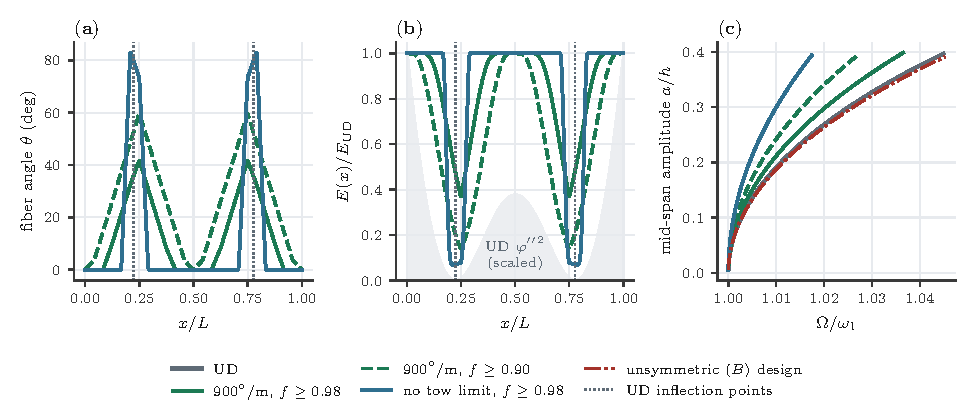
\includegraphics[width=\linewidth]{figs/fig_beam.pdf}
\caption{\textbf{On a symmetric beam, steering flattens the backbone by turning the fibers compliant
where the beam does not bend.} \textbf{(a)}~Optimized mirror-symmetric fiber angle
of the symmetric ($\bm B=\bm0$) clamped beam for three designs: tow limit $900^\circ$/m
with the frequency held to $f\geq0.98$ or $f\geq0.90$ of the UD value, and no tow limit
with $f\geq0.98$. The UD beam ($\theta\equiv0$, $E=E_{\UD}$) appears in (c) only.
\textbf{(b)}~The axial modulus these fields produce, against the UD curvature weight
$\varphi''^2$ that sets $\omega_1^2$ (shaded). Fibers turn compliant where the beam does
not bend: the inflection points (dotted). \textbf{(c)}~Mid-span backbones from the full FE
beam and its cubic SSM; steering flattens the backbone markedly. (The optimized
unsymmetric, $\bm B$-coupled laminate was computed on a different beam model and objective,
so it is compared in the text, not plotted.)}
\label{fig:beam}
\end{figure}

\subsection{The achievable frequency--hardening set of the plate (P3)}\label{sec:levers}
Figure~\ref{fig:levers}a places every design class in the plane
$(\omega_1/\omega_{1,\UD},\,J/J_{\UD})$ at the same mass.

\paragraph{Uniform layups.} A uniform single angle traces a one-parameter curve. As
$\theta$ grows from $0^\circ$ the plate stiffens (up to $\nUfmax\,\omega_{1,\UD}$ at
$90^\circ$, fibers across the short span), and $J$ first falls to $\nUJmin$ at
$\theta=\nUthJmin^\circ$, where $\omega_1=\nUfatJmin\,\omega_{1,\UD}$, then rises. The
$\nSnum$ uniform symmetric stacks on a $15^\circ$ grid fill a region with a global
minimum of $\nSmin$ at $\nSfatmin\,\omega_{1,\UD}$. A grid envelope is not the strongest
uniform competitor: between grid points the continuous single angle already beats it
($\nUEleven$ vs.\ $\nGEleven$ at $1.1\,\omega_{1,\UD}$). We therefore also optimize the
four ply angles of $[\theta_4/\theta_3/\theta_2/\theta_1]_s$ \emph{continuously} at each
held frequency (SLSQP with the frequency equality, 22 starts from the best grid stacks,
the single-angle solution and random stacks; \texttt{stack\_continuous.py}). The best
uniform laminate reaches $J/J_{\UD}=\nCSEleven$, $\nCSTwelve$ and $\nCSThirteen$ at
$1.1$, $1.2$ and $1.3\,\omega_{1,\UD}$.

\paragraph{The UD floor.} Corollary~\ref{cor:udfloor} proves that the lowest-frequency uniform
symmetric laminate of this plate is a single-angle one, and the single-angle sweep shows that it is
UD. The enumeration agrees: the smallest stack frequency is $\nSfmin\,\omega_{1,\UD}$. At
exactly $\omega_1=\omega_{1,\UD}$ the continuous stack optimum is UD itself (all ply angles
$\to0$); the best grid stack within $\pm1\%$ of that frequency, at a slightly different
$\omega_1$, has $J/J_{\UD}=\nSheld$, a negligible difference. For a plate
mandated to the UD frequency, the uniform design space is therefore a single point. This is the one
comparison that is exact for \emph{every} uniform laminate. Above $\omega_{1,\UD}$ the uniform
competitors are the classes we surveyed: all single angles, all $\nSnum$ grid stacks and the
continuously optimized eight-ply stacks. Those comparisons are numerical, not proved bounds.

\paragraph{Steered designs.} At exactly $\omega_{1,\UD}$, the steered single ply reaches
$J/J_{\UD}=\nFTen$, a $\nFTenRed\%$ reduction, with $R_{\min}=\SI{20}{mm}$ imposed (it is active but changes $J$ only in the fourth digit: without
it the optimum is $\nResAInf$, Sec.~\ref{sec:limits}). The steered designs lie well below the best surveyed uniform laminate at
every frequency we test: $\nFEleven$, $\nFTwelve$ and $\nFThirteen$ at $1.1$,
$1.2$ and $1.3\,\omega_{1,\UD}$, against $\nCSEleven$, $\nCSTwelve$ and $\nCSThirteen$
for the best continuous stacks. Steering can also \emph{lower} the frequency below the uniform floor
($\nFNine$ at $0.9\,\omega_{1,\UD}$), which, by Corollary~\ref{cor:udfloor}, no uniform laminate can do. Steering the best
stack at $\omega_{1,\UD}$ gives $\nSFTen$, no better than the steered single ply. For
this plate and objective, the in-plane channel of Sec.~\ref{sec:channels} dominates the
through-thickness channel. Prediction P3 holds with a wide margin: exactly at $\omega_{1,\UD}$,
and against every surveyed uniform class above it.

\begin{figure}[!tbp]
\centering
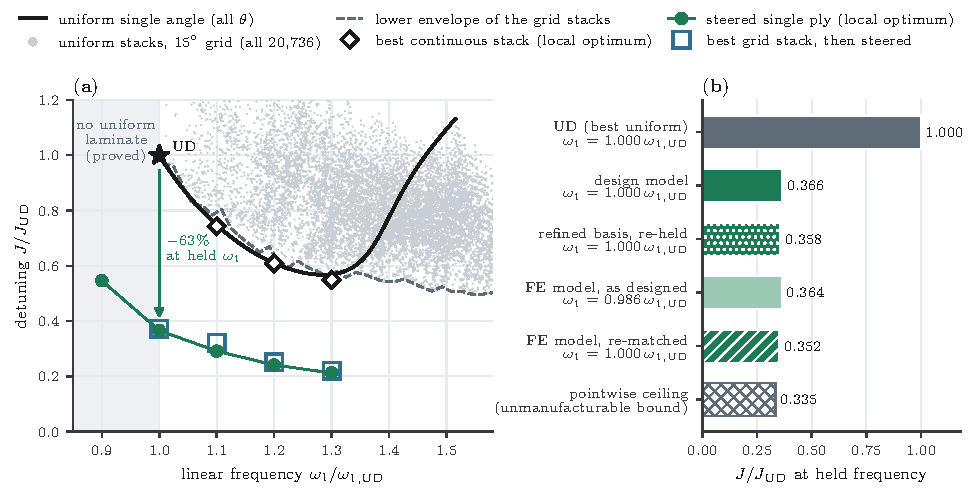
\includegraphics[width=\linewidth]{figs/fig_levers.pdf}
\caption{\textbf{At the unidirectional frequency and mass, steering reaches a hardening that no uniform
symmetric laminate can reach, and above it steering undercuts every uniform class surveyed; the
held-frequency result holds with the frequency re-matched in every model.} \textbf{(a)}~Linear
frequency vs.\ frequency-normalized hardening. Provenance is marked in the legend.
\emph{Proved}: the shaded band $\omega_1<\omega_{1,\UD}$, where no uniform laminate exists
(Corollary~\ref{cor:udfloor}). \emph{Exhaustive}: the uniform single angle (black curve) and all
$\nSnum$ symmetric stacks on a $15^\circ$ grid (gray dots, clipped at $J/J_{\UD}=1.2$; dashed: their
lower envelope). \emph{Local optima}: the best continuous eight-ply stack at each held frequency
(open diamonds, 22 starts), the steered single ply at five target frequencies with
$R_{\min}=\SI{20}{mm}$ (green), and the best grid stack at each target, then steered (blue squares;
none exists at $0.9\,\omega_{1,\UD}$). The arrow marks the held-frequency reduction.
\textbf{(b)}~The held-frequency design's $J/J_{\UD}$ in each model, with the frequency at which it
is evaluated: the design model (equality exact); a refined basis ($m,n\le12$) with the equality
re-imposed; the independent FE model as designed ($\omega_1$ $\nHeldTol\%$ low) and with the
frequency re-matched; the full multi-mode plate's SSM as designed ($\omega_1$ $\nFullAsisPct\%$ high) and
re-matched; and the pointwise ceiling of Sec.~\ref{sec:limits} (unmanufacturable; an estimate). At
$\omega_{1,\UD}$ the best uniform laminate is UD itself; the best grid stack there is UD to within
$\nGridStackDiff\%$ in $J$ ($[0/0/0/15]_s$), and steering it gives $\nSFTen$.}
\label{fig:levers}
\end{figure}

\subsection{The mechanism (P4)}\label{sec:mechanism}
Figure~\ref{fig:mechanism} tests the mechanism of Sec.~\ref{sec:theory} directly.
\begin{itemize}[itemsep=1pt]
\item \textbf{Where the energies live.} Both energies of the UD mode peak at the center.
  The bending energy is concentrated there, with the principal curvature along $y$, across
  the short span, so the held-frequency constraint favors fibers along $x$ there (panel a). The relaxed-stretch energy lies in a band along $x$ through
  the center, with its across-stretch direction along $x$ there and turning toward the
  corners (panel b).
\item \textbf{Sign of the trade-off.} At the held UD frequency the multiplier is negative,
  $\Lambda=\nLambda$ (dimensionless: $e_G$ and $e_K$ normalized by the UD $\gamma$ and
  $\omega_1^2$): minimizing the stretch energy alone would raise the frequency to
  $\nFreeFreq\,\omega_{1,\UD}$, so the constraint pushes the fibers \emph{across} the
  curvature. At the center the two preferences agree (fibers along $x$), and the pointwise design
  $\theta^\star$ keeps the UD direction there.
\item \textbf{Conflict.} Away from the center the across-stretch and across-curvature
  directions separate (panel c); their energy-weighted mean angle is $\nConflict^\circ$.
  This is where a single angle must compromise.
\item \textbf{Pointwise prediction.} The first-order design $\theta^\star(\bm x)$ of
  Proposition~\ref{prop:pointwise}, computed from the UD fields alone with no optimizer
  and no smoothness (panel d), already gives $J/J_{\UD}=\nStarJ$ when evaluated on the
  full model. Its frequency is $\nStarF\,\omega_{1,\UD}$, because the frozen-field model
  ignores the adaptation of the mode.
\item \textbf{Optimized field.} The optimized, curvature-limited field (panel e) shares the
  large-scale pattern of $\theta^\star$ (fibers turned off-axis toward the short edges) but
  departs from it in detail: the energy-weighted RMS angle difference is $\nStarDev^\circ$
  over the plate and $\nStarDevHigh^\circ$ where the energies are large, and at the energy
  peak the optimum is tilted to $\nOptAtPeak^\circ$. The frozen-field design ignores the
  adaptation of the mode and the smoothness and tow limit of a curvature-feasible field, both
  of which the optimizer must respect.
\end{itemize}

Panel f shows which terms move, normalized by UD:
\begin{itemize}[itemsep=1pt]
\item the raw (restrained) membrane cubic falls to $k_{nl}=\nDknl$;
\item the relaxation $2\bm g^{\!\top}\bm K_{\mathrm{in}}^{-1}\bm g$ changes to $\nDrelax$ of
  its UD value, a share of $k_{nl}$ rising from $\nRelaxUD\%$ to $\nRelaxOpt\%$;
\item the relaxed cubic falls to $\gamma=\nDgamma$;
\item the frequency is held ($\omega_1^2=\nDomsq$) and the mode's center value changes to
  $w_c=\nDmid$.
\end{itemize}
The hardening falls mainly through the direct term of \eqref{eq:gamma}: fibers across the
principal stretch store less membrane energy for the same stretch, so $k_{nl}$ falls to
$\nDknl$ of its UD value. The relaxation falls less (to $\nDrelax$), so its share of the
stretch energy rises and $\gamma$ falls further than $k_{nl}$ alone. Prediction P4 holds
partly: $\theta^\star$ alone captures most of the gain, though at $\nStarF\,\omega_{1,\UD}$, but the optimum departs from it by $\nStarDevHigh^\circ$ RMS even where the
energies are large.

\begin{figure}[!tbp]
\centering
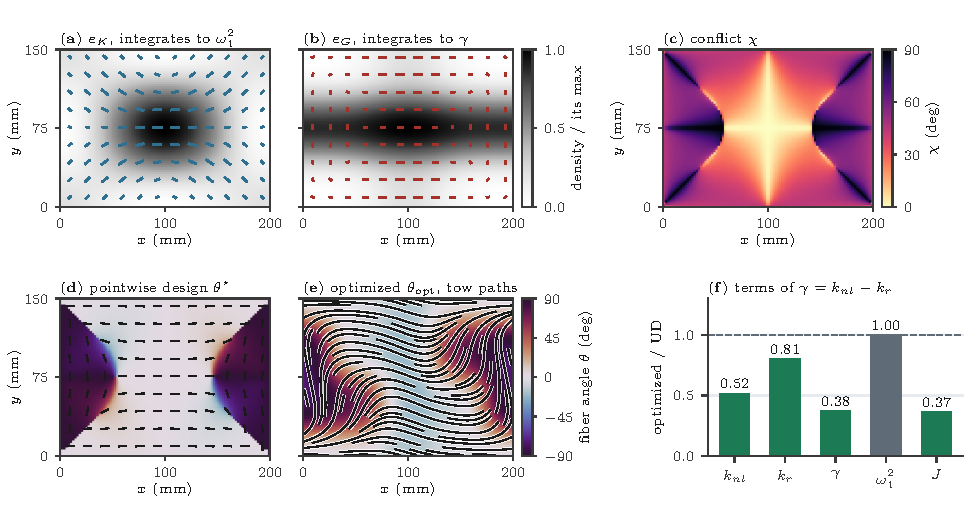
\includegraphics[width=\linewidth]{figs/fig_mechanism.pdf}
\caption{\textbf{The two energies prefer different fiber directions away from the plate
center; the optimized field follows a compromise that a single angle cannot make.} All maps show the
full $\SI{200}{mm}\times\SI{150}{mm}$ plate with the same axes; angles are measured from the $x$
axis. \textbf{(a)}~Bending-energy density $e_K$ of the UD fundamental, which integrates to
$\omega_1^2$. Blue ticks: the fiber direction the held-frequency constraint favors ($\Lambda<0$:
across the principal curvature, $\varphi_K+90^\circ$). \textbf{(b)}~Relaxed-stretch density $e_G$,
which integrates to $\gamma$, on the same normalized gray scale. Red ticks: the direction that
minimizes it (across the principal stretch, $\varphi_G+90^\circ$). Tick length in (a) and (b)
scales with the local anisotropic amplitude. \textbf{(c)}~Conflict $\chi$, the angle between the
ticks of (a) and (b). It vanishes at the center and along the central cross ($x=\SI{100}{mm}$, and
$y=\SI{75}{mm}$ for $60<x<\SI{140}{mm}$), where one direction serves both energies, and reaches $90^\circ$
along $y=\SI{75}{mm}$ near the short edges. The sharp ridges are lines where one of the two principal directions is undefined
(equal principal strains). \textbf{(d)}~First-order pointwise design $\theta^\star$ from the UD
fields alone (Proposition~\ref{prop:pointwise}); black ticks: the same direction field.
\textbf{(e)}~Optimized curvature-limited field; colors give the fiber angle and black lines the tow
paths. (d) and (e) share one cyclic color scale, lightest at $\theta=0^\circ$.
\textbf{(f)}~Optimized/UD ratios of the terms of \eqref{eq:gamma}: the restrained cubic $k_{nl}$,
the relaxation $k_{r}=2\bm g^{\!\top}\bm K_{\mathrm{in}}^{-1}\bm g$, their difference $\gamma$,
$\omega_1^2$ (held) and $J$; dashed: parity with UD.}
\label{fig:mechanism}
\end{figure}

\subsection{What bounds the lever (P5)}\label{sec:limits}
\paragraph{Anisotropy.} Along the family $\bm Q(s)=\bm Q_{\mathrm{iso}}+s(\bm Q-\bm
Q_{\mathrm{iso}})$, which keeps the isotropic invariants $U_1,U_4,U_5$ and scales $U_2,U_3$
by $s$, the held-frequency steered optimum falls monotonically with the anisotropy:
\begin{itemize}[itemsep=1pt]
\item $J/J_{\UD}=\nDoseA$ at $E_1/E_2=\nDoseRatioA$;
\item $\nDoseC$ at $\nDoseRatioC$;
\item $\nDoseE$ at $\nDoseRatioE$ (CFRP);
\item $\nDoseF$ at $\nDoseRatioF$ (Fig.~\ref{fig:limits}a).
\end{itemize}
The isotropic limit has no lever (Corollary~\ref{cor:iso}).

\paragraph{Tow curvature.} The held-frequency optimum degrades smoothly as the minimum
tow radius grows:
\begin{itemize}[itemsep=1pt]
\item $\nFrontThirty$ at $R_{\min}=\SI{30}{mm}$;
\item $\nFrontFifty$ at $\SI{50}{mm}$;
\item $\nFrontEighty$ at $\SI{80}{mm}$;
\item $\nFrontOneFifty$ at $\SI{150}{mm}$;
\item $\nFrontFourHundred$ at $\SI{400}{mm}$ (Fig.~\ref{fig:limits}b).
\end{itemize}
Below $R_{\min}\approx\SI{20}{mm}$ it saturates at $\nFrontTwenty$. Two checks show that
the saturation is physical rather than an artifact of the 50\,mm support grid.
\begin{itemize}[itemsep=1pt]
\item \textbf{Finer grid.} Refining the grid to 33\,mm and 25\,mm changes the optimum
  only to $\nResBTwenty$ and $\nResCTwenty$ at $R_{\min}=\SI{20}{mm}$, and to
  $\nResBInf$ and $\nResCInf$ with no tow limit.
\item \textbf{Pointwise ceiling.} Freeing $\theta$ at every quadrature point, with no
  smoothness and no tow limit, gives $\nCeil$. This field cannot be laid, and it is the best
  local optimum found for a nonconvex problem, so it estimates rather than bounds what
  single-ply steering can reach.
\end{itemize}
The plate's strain fields vary on a length scale of a few centimeters. Once tows can
turn on that scale, further manufacturing freedom buys little. The front of
Fig.~\ref{fig:limits}b is the best design found from six starts at each radius, so the attainable
front lies at or below it; the pointwise ceiling indicates how much lower it could plausibly go. Prediction P5 holds:
the lever is set by the material anisotropy and by the ratio of the tow radius to the
length scale of the mode's strain fields. Its third ingredient, the conflict between the two
fields, is tested across plates in Sec.~\ref{sec:robust}.

\begin{figure}[!tbp]
\centering
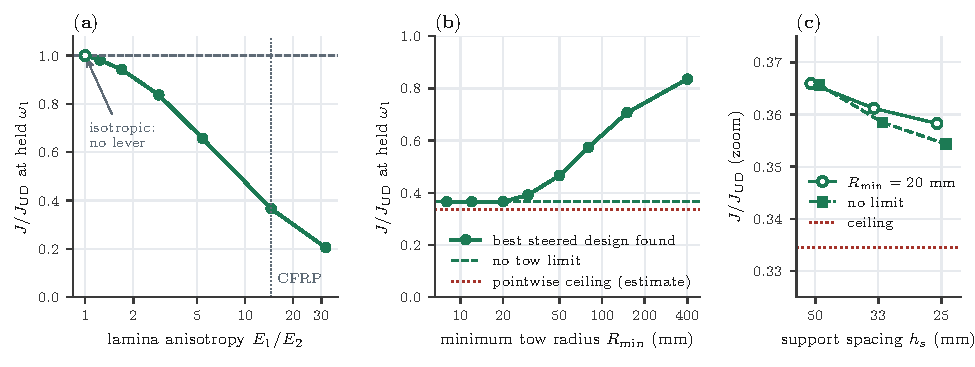
\includegraphics[width=\linewidth]{figs/fig_limits.pdf}
\caption{\textbf{The lever vanishes for isotropic material, grows with anisotropy, and saturates
once tows can turn on the strain-field length scale.} All at held frequency. \textbf{(a)}~Steered optimum vs.\
lamina anisotropy along a family that scales only the anisotropic invariants
($E_1/E_2=1$ is isotropic, where $J/J_{\UD}=1$ exactly by Corollary~\ref{cor:iso}, so that point is
not computed; dashed: parity with UD; dotted: CFRP). \textbf{(b)}~Tow-radius front: best design found vs.\ minimum tow
radius on the 50\,mm support grid; dashed: the same grid with no tow limit; dotted: the
pointwise ceiling (unconstrained, unsmoothed; an estimate, not a bound). Each point is the best of six
starts.
\textbf{(c)}~Support-grid refinement (zoomed
ordinate; the three support spacings are plotted as equally spaced categories, with the two
series offset slightly for visibility): at $R_{\min}=\SI{20}{mm}$ (open) and with no tow limit (filled) the optimum
moves by less than $0.02$ and approaches the ceiling, so the saturation in (b) is physical,
not a parametrization artifact.}
\label{fig:limits}
\end{figure}

\subsection{Independent confirmation on the full model}\label{sec:confirm}
The design was produced on the condensed, adapted-mode evaluator. We confirm it on the
full multi-mode plate: 36 transverse and 72 in-plane modes, in-plane inertia retained,
an independent Gauss-quadrature assembly, and amplitudes measured as the true mid-plate
deflection (Table~\ref{tab:confirm}).
\begin{itemize}[itemsep=1pt]
\item \textbf{Full SSM.} The full cubic SSM gives detuning coefficients $\beta$ within
  $\nSSMvsEval\%$ of the evaluator for both designs. The detuning ratio is $\nCratioSSM$, a
  $\nCredSSM\%$ reduction.
\item \textbf{EPMC.} Full-order EPMC continuation ($H=\nEPMCH$ harmonics) gives a ratio of $\nCratioEPMC$.
\item \textbf{Frequency.} The steered design's full-model frequency is $\nCOptf$\,Hz
  against $\nCUDf$\,Hz for UD. The difference is the Ritz upper-bound convergence of the
  transverse basis for the steered field (Table~\ref{tab:conv}: the steered frequency
  falls by $\nConvFreqDrop\%$ from $m,n\le8$ to $m,n\le16$ while the UD frequency is unchanged), not a
  design change.
\item \textbf{Discretization.} An independent finite-element model (ACM Kirchhoff
  bending with Q4 membrane elements, Appendix~\ref{app:fe}) evaluated on the optimized
  field gives a detuning ratio of $\nFEratio$. Across the three discretizations the
  steered design's frequency lies within $\pm\nHeldTol\%$ of the UD value.
\end{itemize}

\paragraph{Matched-frequency comparison.} In the refined design basis and in the FE model the steered
frequency comes out slightly \emph{below} the UD value, which is unfavorable to steering because $J$ falls
as the frequency rises along the steered front (Fig.~\ref{fig:levers}a). In the full multi-mode plate it
comes out $\nFullAsisPct\%$ \emph{above}, which favors it. To remove the drift in both directions rather
than bound it, we re-impose the equality in each model (\texttt{r1\_\allowbreak matched\_\allowbreak
frequency.py}, \texttt{r1\_\allowbreak full\_\allowbreak matched.py}; Fig.~\ref{fig:levers}b).
\begin{itemize}[itemsep=1pt]
\item \textbf{Refined basis.} On $m,n\le12$ (144 transverse and 128 in-plane modes) the published design
  has $\omega_1=\nRefEvalF\,\omega_{1,\UD}$ and $J/J_{\UD}=\nRefEvalJ$. Re-solving the held-frequency
  problem on that basis, with the equality exact, gives $J/J_{\UD}=\nRefHeldJ$.
\item \textbf{Independent FE model.} The design as laid has $\omega_1=\nFEasisF\,\omega_{1,\UD}$ and ratio
  $\nFEasisJ$. We move it along the design model's frequency-gradient direction until the FE
  frequencies agree to $10^{-5}$ (a one-parameter move, not a re-optimization, so conservative). The ratio
  is then $\nFEmatchedJ$. Along that path
  $\dd(J/J_{\UD})/\dd(\omega_1/\omega_{1,\UD})=-\nFEslope$, so a frequency drift of $1\%$ moves the
  headline ratio by less than $0.01$.
\item \textbf{Full multi-mode plate.} Moved in the same way until its linear frequency equals the UD
  value to $10^{-6}$, the steered design has an SSM detuning ratio of $\nFullMatchedJ$ (as designed:
  $\nCratioSSM$) and an EPMC ratio of $\nFullMatchedEPMC$.
\end{itemize}
The held-frequency result is therefore not an artifact of the design discretization. With the
frequency matched in each model, the steered plate is at $\nFEmatchedJ$--$\nFullMatchedEPMC$ of the UD
hardening.

\begin{table}[!tbp]
\centering\footnotesize
\caption{Confirmation of the held-frequency design. $\beta$: small-amplitude coefficient
of $\Om/\omega_1-1=\beta(a/h)^2$ at the plate center.}\label{tab:confirm}
\begin{tabular}{@{}lcccc@{}}
\toprule
model & $f_1$ UD (Hz) & $f_1$ steered (Hz) & $\beta$ UD & $\beta$ steered\\ \midrule
design evaluator (64+72 modes, condensed) & $\nUDf$ & $\nUDf$ & $\nEvBetaUD$ & $\nEvBetaOpt$\\
full plate, cubic SSM (36+72 modes) & $\nCUDf$ & $\nCOptf$ & $\nCUDbetaSSM$ & $\nCOptbetaSSM$\\
full plate, EPMC ($H=\nEPMCH$) & --- & --- & $\nCUDbetaEPMC$ & $\nCOptbetaEPMC$\\
independent FE (ACM + Q4, $\nFEmesh$, App.~\ref{app:fe}) & $\nFEUDf$ & $\nFEOptf$ & $\nFEUDbeta$ & $\nFEOptbeta$\\
\bottomrule
\end{tabular}
\end{table}

\subsection{Consequence: a wider jump-free range}\label{sec:jumpres}
The backbone improvement (Secs.~\ref{sec:levers}--\ref{sec:confirm}) is a property of the
conservative system. Turning it into a forced-response statement needs a damping model and a
forcing, so the absolute numbers below are specific to the model ($\zeta=2\%$ mass-proportional, a
center point load). The \emph{ratio} of jump-free amplitudes is not: Proposition~\ref{prop:cusp}
predicts that the held-frequency reduction widens the jump-free amplitude by
$(J_{\mathrm{steered}}/J_{\UD})^{-1/2}=\nCacTheory$, whatever $\zeta$ is, and
Sec.~\ref{sec:robust} tests that independence. We compute
$a_c$ numerically as the drive at which the full-order damped SSM forced response
($\zeta=2\%$, center point load) first becomes multivalued. It rises from $a_c/h=\nCUDac$
to $\nCOptac$, a factor $\nCacRatio$ in amplitude and $\nCFratio$ in drive. This agrees
with the predicted ratio, and the absolute thresholds agree too: \eqref{eq:ac} with the
full-model $\beta$ gives $\nCacFormUD$ and $\nCacFormOpt$.

Direct time integration then shows the jump itself (Fig.~\ref{fig:confirm}b,c). We drive
both panels with the same point load, set between their two thresholds, and sweep the
frequency up and down. The UD panel is hysteretic: the up and down sweeps differ by up
to $\nCUDgap\,h$ across the fold. The steered panel, at the same frequency and mass, is
single-valued: its sweeps coincide to $\nCOptgap\,h$ and follow the SSM forced response. A finer
sweep ($\nFineSteps$ steps over $\Om/\omega_1\in[1.00,1.08]$; \texttt{confirm\_\allowbreak fine\_\allowbreak sweep.py})
confirms both: the UD up and down sweeps differ at $\nFineHyst$ consecutive steps across the
fold (by up to $\nFineGap\,h$), the steered sweeps at none.
\begin{figure}[!tbp]
\centering
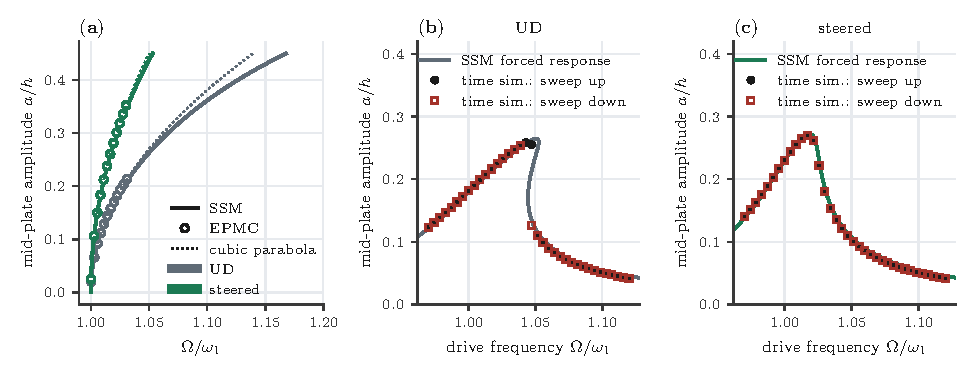
\includegraphics[width=\linewidth]{figs/fig_confirm.pdf}
\caption{\textbf{The full model confirms the reduction, and at one drive the UD panel jumps while the
steered panel, at the same frequency and mass, does not.} \textbf{(a)}~Free mid-plate backbones of the
full multi-mode plate (36 transverse + 72 in-plane modes): cubic SSM (lines) and full-order EPMC with
$H=\nEPMCH$ harmonics (marks; squares UD, circles steered). Dotted: the cubic parabola
$1+\beta(a/h)^2$ with the full-model SSM $\beta$ (within $\nSSMvsEval\%$ of the condensed evaluator's).
\textbf{(b,c)}~Forced response at one drive between the two jump thresholds ($\zeta=2\%$, center point
load): full-plate damped SSM (line) and direct time integration of up sweeps (black dots) and down sweeps
(red squares) on a six-mode modal model, 300 forcing periods per step. A point is kept once its
amplitude is steady to $0.4\%$, which excludes one UD point at the fold.}
\label{fig:confirm}
\end{figure}

\subsection{Robustness of the lever}\label{sec:robust}
The result above is for one plate, one support, one damping law and an idealized laminate. This
section varies each in turn (Fig.~\ref{fig:robust}).

\paragraph{Other plates and the conflict test of P5.} We solve the same held-frequency problem
($R_{\min}=\SI{20}{mm}$, 50\,mm support grid, six starts) for a square and a 2:1 plate, for clamped
edges, and for in-plane traction-free edges, and compare each with the strongest uniform laminate at
the same frequency (all single angles and a continuous eight-ply stack optimization;
\texttt{r1\_\allowbreak generality.py}).
\begin{itemize}[itemsep=1pt]
\item \textbf{Aspect ratio.} The steered optimum is $J/J_{\UD}=\nGenSqJ$ on the square plate and
  $\nGenTwoJ$ on the 2:1 plate, against $\nGenBaseJ$ on the paper's 4:3 plate. On all three the UD
  plate is again the lowest-frequency uniform laminate, so UD is the best uniform design at
  $\omega_{1,\UD}$.
\item \textbf{Clamped edges.} Here UD is \emph{not} the frequency floor: the lowest uniform frequency,
  $\nGenClMinF\,\omega_{1,\UD}$, occurs at a single angle of $\nGenClMinAng^\circ$, as
  Corollary~\ref{cor:udfloor} allows. A real uniform competitor therefore exists at $\omega_{1,\UD}$. It
  reaches $\nGenClUnif$, and the steered field reaches $\nGenClJ$.
\item \textbf{In-plane movable edges.} With traction-free in-plane edges the UD plate hardens
  $\nGenMvRatio$ times less, because $\nGenMvRelaxUD\%$ of its stretch energy relaxes. Steering still
  halves what remains ($\nGenMvJ$), raising the relaxed share to $\nGenMvRelaxOpt\%$.
\end{itemize}
The lever is general, but its size varies by a factor of three, and the mechanism says why.
Proposition~\ref{prop:pointwise} predicts that steering gains least where the two strain fields share
their principal directions. The energy-weighted conflict $\chi$ of each UD plate
(\texttt{r1\_\allowbreak conflict.py}) orders the results: $\nChiTwo^\circ$ on the 2:1 plate, whose
fundamental bends nearly cylindrically across the short span ($\nGenTwoJ$); $\nChiBase^\circ$ on the
4:3 plate ($\nGenBaseJ$); and $\nChiSq^\circ$ on the square plate ($\nGenSqJ$). The clamped
($\nChiCl^\circ$) and movable-edge ($\nChiMv^\circ$) plates fall near the same trend
(Fig.~\ref{fig:robust}b). The test is suggestive rather than decisive. The conflict was added to P5
in this revision, only three simply supported plates order it, and another property of the UD fields,
the frequency that minimizing the stretch energy alone would select ($\nFreeFreqTwo$, $\nFreeFreq$ and
$\nFreeFreqSq\,\omega_{1,\UD}$ for the three plates), orders them equally well. The 2:1 value is also
limited by the support grid, which has only three rows across its 100\,mm span: refining the grid to
33\,mm and 25\,mm lowers it to $\nGridTwoB$ and $\nGridTwoC$, against $2\%$ on the 4:3 plate. The ordering
of the plates is unchanged.

\paragraph{Damping level and law.} We recompute the jump-free amplitude of both designs on the full
damped SSM (\texttt{r1\_\allowbreak damping.py}) for mass-proportional damping $\zeta=0.5$, $1$, $2$
and $4\%$, and for stiffness-proportional damping at $2\%$. The absolute thresholds scale as
$\zeta^{\nDampScale}$ (UD: $a_c/h=\nDampAcLo$ to $\nDampAcHi$), as Proposition~\ref{prop:cusp}'s
$\zeta^{1/2}$ predicts. The steered/UD ratio is $\nDampRatioMin$--$\nDampRatioMax$ for every
mass-proportional level and $\nDampStiffRatio$ for stiffness-proportional damping
(Fig.~\ref{fig:robust}c). Two caveats apply. With mass-proportional damping the cubic damped SSM is the
model for which Proposition~\ref{prop:cusp} is exact, so the constancy of the ratio there is largely a
consistency check; the stiffness-proportional case, whose decay rate depends on amplitude through the
mode, is the independent test. And at $\zeta=4\%$ the thresholds ($a_c/h=\nDampAcHi$ for UD,
$\nDampAcHiOpt$ steered) exceed the amplitude range over which the cubic SSM is verified against EPMC
($a/h\le\nEPMCmaxUD$ and $\le\nEPMCmaxOpt$), so those two points are cubic-model predictions only.
Within those limits, the widening of the jump-free range is a property of the hardening, not of the
damping model.

\paragraph{As built.}\label{sec:asbuilt} The designs are idealized tow fields
(Sec.~\ref{sec:intro}). Laying them with tows of constant width along the tow paths changes the local
tow density, because neighboring paths spread or converge at the rate
$\dd\ln(\text{spacing})/\dd\ell=\nabla\!\cdot\bm n$, with $\bm n=(\cos\theta,\sin\theta)$. A course
that starts fully covering its inflow edge reaches $\bm x$ with relative density
$\tau(\bm x)=\exp(-\int\nabla\!\cdot\bm n\,\dd\ell)$, integrated back along the path
(\texttt{r1\_\allowbreak asbuilt.py}). For the held-frequency design $\tau$ spans $\nTauMin$ to
$\nTauMax$ (Fig.~\ref{fig:robust}d). Uncut courses are therefore not an option: they would leave
$\nTauGapArea\%$ of the plate thinned. In a constant-tow-count model (thickness $h\tau$, as in continuous
tow shearing \cite{kim2012}) the frequency would fall to $\nCtsF\,\omega_{1,\UD}$ at $\nCtsM$ of the mass, and
$J/J_{\UD}$ would rise to about $\nCtsJ$. The field requires tow cut/add. With cut/add inside courses of $N$ tows, the coverage mismatch at a course
boundary never exceeds one tow width and averages half of one. We model this, in the spirit of the
defect-layer method \cite{fayazbakhsh2013}, as a defect area fraction
$f_d=\tfrac{1}{2N}\min\!\big(1,|\ln\tau|/\ln(1+1/N)\big)$. It is either resin-filled gaps (0\%
coverage: constant thickness, fiber fraction $1-f_d$) or overlaps (100\% coverage: thickness
$1+f_d$). Fig.~\ref{fig:robust}e places the results in the frequency--hardening plane.
\begin{itemize}[itemsep=1pt]
\item With $N=8$ tows per course, gaps give $J/J_{\UD}=\nGapEightJ$ at $\nGapEightF\,\omega_{1,\UD}$
  (mass $\nGapEightM\%$), and overlaps give $\nOvlEightJ$ at $\nOvlEightF\,\omega_{1,\UD}$ (mass
  $\nOvlEightM\%$).
\item Over $N=4$--$16$, $J/J_{\UD}$ stays between $\nAsBuiltJmin$ and $\nAsBuiltJmax$, but the frequency and
  mass are no longer held: the frequency ranges over $\nAsBuiltFmin$--$\nAsBuiltFmax\,\omega_{1,\UD}$ and the mass
  over $\nAsBuiltMmin$--$\nAsBuiltMmax$ of UD. The lowest ratio, $\nAsBuiltJmin$, belongs to the heaviest and
  stiffest variant (overlaps, $N=4$). The as-built points lie near the steered front of the idealized
  designs, which is computed at fixed mass, so the comparison with that front is indicative only.
\item A smooth random angle error of $2^\circ$ RMS (correlation length 25\,mm, 40 samples) gives
  $J/J_{\UD}=\nAngJmean\pm\nAngJstd$, with a frequency scatter of $\nAngFstd\%$.
\end{itemize}
Defects mainly shift the frequency and mass and leave $J/J_{\UD}$ near the steered front; the
defect model, in particular its cap $f_d\le1/(2N)$, is an assumption that largely sets this result. A buildable design at an exactly held frequency would put the defect model
inside the optimization, which is beyond the present scope (Sec.~\ref{sec:discussion}).

\paragraph{The optimizer.} The analytic gradients of $J$, $\omega_1$, $\gamma$ and the tow curvature agree
with central finite differences to better than $\nGradErr$ relative along $\nGradDirs$ directions. The
final field's tow curvature, re-evaluated on an independent 1\,mm grid, gives a minimum radius of
$\nRminFine$\,mm against the 20\,mm limit (an excess of $\nKappaOver\%$ between quadrature points). Of
the six starts, $\nMSgood$ reach within $\nMSspread\%$ of the best design and two stall at up to
$\nMSworst$ (Table~\ref{tab:ms}). The local optimizer can stall, and the reported optimum is the best
of the starts (\texttt{r1\_\allowbreak verification.py}).

\begin{figure}[!tbp]
\centering
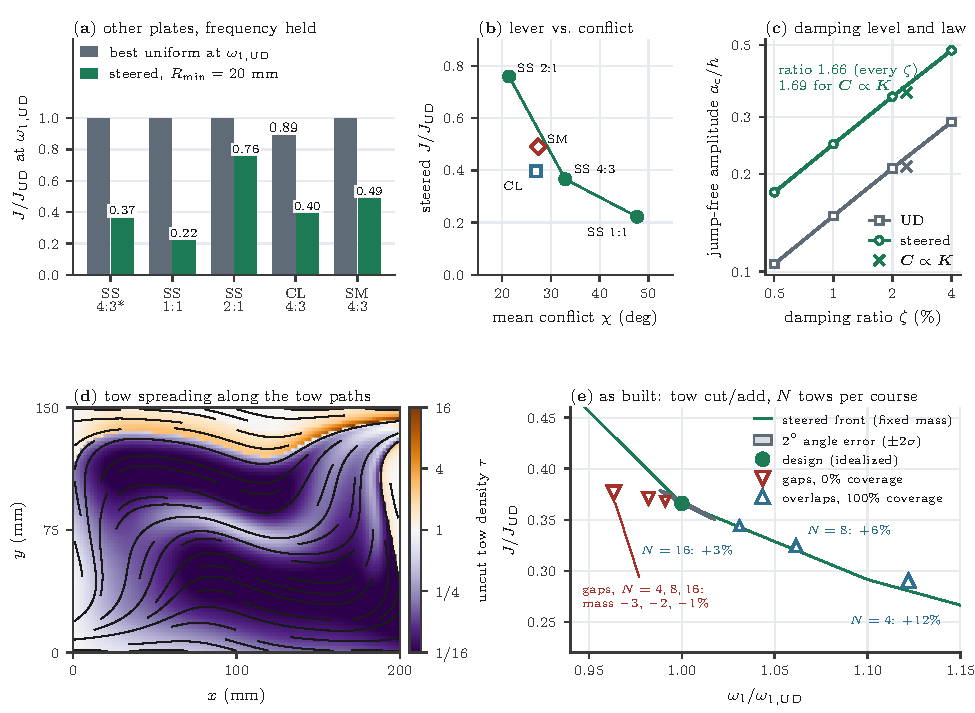
\includegraphics[width=\linewidth]{figs/fig_robust.pdf}
\caption{\textbf{The lever persists across plates, supports, damping laws and as-built defects, and its size
is ordered by the conflict between the two strain fields.} \textbf{(a)}~Held-frequency $J/J_{\UD}$ of
the steered optimum (green) and of the best uniform laminate at the same frequency (gray) for simply
supported (SS) plates of aspect ratio 4:3 (the paper's plate, $\ast$), 1:1 and 2:1, a clamped plate
(CL) and a simply supported plate with in-plane movable edges (SM). Each plate is normalized by its
own UD design; only the clamped plate has a uniform competitor other than UD at $\omega_{1,\UD}$.
\textbf{(b)}~Steered optimum vs.\ the energy-weighted conflict $\chi$ of the UD fields; line: the three
SS plates. \textbf{(c)}~Jump-free amplitude $a_c/h$ from the full damped SSM vs.\ damping ratio
(mass-proportional, lines; stiffness-proportional at $\zeta=2\%$, crosses, drawn slightly to the right for
visibility). Both designs scale as $\zeta^{1/2}$, and
their ratio does not change. \textbf{(d)}~Relative density $\tau$ of uncut constant-width tows laid
along the tow paths of the held-frequency design (black lines). Purple: spreading (gaps if uncut);
orange: convergence (overlaps); color scale clipped at $1/16$ and $16$ ($\tau$ spans
$\nTauMin$--$\nTauMax$). \textbf{(e)}~As-built laminates with tow cut/add, $N=4$, $8$, $16$ tows per course
(labels: $N$ and the mass change): resin gaps (down triangles), overlaps (up triangles), and a $2^\circ$ RMS
angle error (gray ellipse: mean $\pm2$ standard deviations). Their mass differs from UD, unlike the steered
front, which is at fixed mass.}
\label{fig:robust}
\end{figure}

\section{Discussion}\label{sec:discussion}

\subsection{Answer to the question}
\begin{itemize}[itemsep=1pt]
\item \textbf{Can steering do it?} Yes. At the frequency (held exactly in the design
  model, to within $\nHeldTol\%$ on refined bases and an independent finite-element model) and mass of the unidirectional plate, a manufacturable steered tow reduces the frequency-normalized
  hardening by $\nFTenRed\%$. No uniform layup can reach that frequency at a lower
  hardening, and steering undercuts the best stacking sequences at every higher
  frequency we test.
\item \textbf{Why?} The frequency and the hardening read the same rotated stiffness
  through two strain fields whose principal directions turn differently over the plate,
  and an optimal design must satisfy the trade-off between them pointwise
  (Proposition~\ref{prop:pointwise}).
\item \textbf{What bounds it?} The material anisotropy ($U_2,U_3$), and the tow radius
  relative to the length scale of the fields.
\item \textbf{How does it compare?} Steering is the stronger channel here. It is also
  the one that does not require changing the bill of materials.
\end{itemize}

\begin{table}[h]
\centering\footnotesize
\caption{Status of the predictions.}\label{tab:verdict}
\begin{tabular}{@{}p{0.39\linewidth}p{0.39\linewidth}p{0.13\linewidth}@{}}
\toprule
prediction & evidence & verdict\\ \midrule
P1 isotropic material has no lever & Cor.~\ref{cor:iso}; gradient $\equiv0$ to $10^{-10}$; Fig.~\ref{fig:limits}a & holds (exact)\\
P2 uniform angle cannot change a single-ply beam; steering can, at the inflection points & SSM ratio $\nBUnif$; Tab.~\ref{tab:beam}; Fig.~\ref{fig:beam} & holds\\
P3 steered plate reaches $(\omega_1,J)$ no uniform layup reaches & Fig.~\ref{fig:levers}; $\nSnum$ stacks & holds\\
P4 optimized field follows preferred directions; $\theta^\star$ captures most of the gain & Fig.~\ref{fig:mechanism}; $\theta^\star$: $\nStarJ$ at $\nStarF\,\omega_{1,\UD}$; optimum departs by $\nStarDevHigh^\circ$ RMS where energies are large & holds partly\\
P5 lever grows with anisotropy, saturates at the field length scale & Fig.~\ref{fig:limits} & holds\\
consequence: $a_c$ widens as $J^{-1/2}$ & $\nCacRatio$ vs.\ $\nCacTheory$; time-domain sweeps & holds\\
\bottomrule
\end{tabular}
\end{table}

\subsection{What is new}
\begin{itemize}[itemsep=1pt]
\item \textbf{Design variable.} Reduced-order optimization of nonlinear dynamics
  \cite{pozzi2024lsm,pozzi2025,pozzi2025smo,liang2025,xiao2026} has used shape, size, density or other system parameters. We use a
  manufacturable fiber-orientation field.
\item \textbf{Objective.} Variable-stiffness composites \cite{gurdal,ijsselmuiden} have been
  steered for linear objectives and for postbuckling \cite{wu2013,raju2018}, and for the
  linear frequency with the nonlinear response examined afterwards
  \cite{farsadi2021,farsadi2025}. We steer them for the hardening itself, at fixed linear
  frequency.
\item \textbf{Mechanism, not only an optimum.} The paper's main contribution is the
  mechanism: a local Fourier theory that predicts when steering must help, where the
  fibers should go, and what limits the gain, tested prediction by prediction.
\item \textbf{Analysis versus design.} Nonlinear vibrations of variable-stiffness plates
  have been computed for prescribed fiber paths
  \cite{ribeiro2012,ribeiroakhavan2012,akhavan2015,akhavan2017,houmat2013,yan2021}. Here
  the path is designed at a held frequency, and the reason it works is identified.
\item \textbf{One-dimensional result.} On a clamped beam the operative lever is not the
  bending--extension coupling but the harmonic-versus-curvature-weighted mean of
  Proposition~\ref{prop:beam}, which requires no coupling at all.
\end{itemize}

\subsection{Limitations and scope}
\begin{itemize}[itemsep=2pt]
\item \textbf{Geometry and support.} Results are for a simply supported, immovable-edge
  rectangular plate. The mechanism is general, but the numbers depend on where the
  curvature and the stretch live, which other supports change.
\item \textbf{Constant thickness.} We assume constant thickness and mass. Real AFP
  steering produces tow gaps or overlaps whose thickness and stiffness changes are not
  modeled. Including them, through a thickness field tied to $\theta(\bm x)$, is the main
  step toward a buildable design.
\item \textbf{Amplitude range.} The design quantity is the small-amplitude cubic
  coefficient. The cubic SSM reproduces the full-order EPMC detuning to within $\nEPMCAgree\%$
  over the amplitudes EPMC reached ($a/h\le\nEPMCmaxUD$ for UD, $\le\nEPMCmaxOpt$ for the steered design),
  and the jump-onset amplitudes reported lie inside these ranges. Higher
  amplitudes need the quintic SSM or EPMC (Appendix~\ref{app:calib}).
\item \textbf{Single mode, no internal resonance.} On the full multi-mode plate the steered design's lowest
  frequencies are in ratios $\nModeRatios$ (\texttt{mode\_\allowbreak ratios.py}). The nearest
  commensurability ($3{:}1$ with the third mode) is detuned by $\nDetThreeOne\%$, and that mode
  is antisymmetric about the center. The $r=6$ mode time-domain model contains these modes
  and would show an internal-resonance exchange; its sweeps follow the single-mode forced
  response instead (Fig.~\ref{fig:confirm}b,c).
\item \textbf{Optimality.} The optimizer is local (multi-start SLSQP). The pointwise
  ceiling of Sec.~\ref{sec:limits} bounds what any single-ply field can do. Stacks have eight
  plies (four independent angles), optimized continuously at each held frequency; more
  plies or a lamination-parameter search could lower the uniform optimum further; the
  steered values are at most $\nSteerVsUniformMax\%$ of the present one. The UD floor at
  $\omega_{1,\UD}$ holds for every uniform laminate (Corollary~\ref{cor:udfloor}).
\item \textbf{Damping.} Damping is fixed ($2\%$ of critical, mass-proportional) and not designed.
\item \textbf{Idealized laminate.} The plate designs are a single $2$\,mm steered ply,
  i.e.\ an unbalanced laminate, and tow gaps and overlaps are ignored. The beam design
  with no tow limit turns to about $\nBeamMaxAngle^\circ$ in narrow zones of the $20$\,mm-wide strip.
\end{itemize}

\subsection{Outlook}
The same reduction and adjoint carry over directly to three extensions:
\begin{itemize}[itemsep=1pt]
\item \emph{prescribing} the backbone (a target frequency--amplitude law) instead of
  minimizing the hardening;
\item adding a density field, so that topology and tow path are designed together;
\item steering stability boundaries, such as supersonic panel flutter, whose
  nonsymmetric aeroelastic operator enters the same first-order pencil; the flutter and
  post-flutter response of plates with prescribed curvilinear fibers has been analyzed
  \cite{akhavan2018,akhavan2020,farsadi2019}, but not designed.
\end{itemize}
The mechanism of Sec.~\ref{sec:theory} predicts where each extension should help: wherever
two functionals of the same stiffness are weighted by different strain fields.

\section{Conclusions}\label{sec:conclusions}
\begin{enumerate}[itemsep=2pt]
\item The frequency and the geometric hardening of a laminated panel integrate the same
  rotated stiffness against the curvature and the relaxed stretch of the fundamental.
  Each density depends on the local fiber angle only through $U_2$, $U_3$ and the local
  principal directions (Proposition~\ref{prop:fourier}).
\item A uniform single angle cannot change the frequency-normalized hardening of a
  single-ply beam. Symmetric steering cuts it by up to $\nBInfHeldRed\%$ with the
  frequency within $\nBeamFreqBand\%$ of the UD value, by placing compliant fibers at the inflection points. In our comparison
  bending--extension coupling was a minor lever ($\nBBred\%$ on its own drift objective,
  against $\nBNineNinetyRed\%$ for symmetric steering at the same $900^\circ$/m tow limit and
  frequency floor); a richer coupled parametrization might do better.
\item On a simply supported plate, a curvature-feasible steered field reduces the
  frequency-normalized hardening by $\nFTenRed\%$ at the unidirectional frequency
  (held exactly in the design model, to within $\nHeldTol\%$ on refined bases and an independent finite-element model) and mass. This point is unreachable by any uniform layup, and the steered
  designs undercut the best stacking sequences at every frequency tested.
\item A pointwise design from the UD fields alone captures most of the gain; the
  optimized field shares its large-scale pattern but not its detail. Steering lowers the restrained stretch energy $k_{nl}$ to $\nDknl$ of its UD
  value; the relaxation falls less ($\nDrelax$), so its share of the stretch energy rises
  ($\nRelaxUD\%\to\nRelaxOpt\%$) and $\gamma$ falls further than $k_{nl}$.
\item The lever vanishes for isotropic material, grows monotonically with anisotropy, and
  saturates once the minimum tow radius is below about $\SI{20}{mm}$.
\item The full-order model confirms the reduction (SSM, EPMC, time integration), and the
  jump-free amplitude widens by $\nCacRatio\times$, in agreement with
  $a_c\propto J^{-1/2}$.
\end{enumerate}

\paragraph{Data and code availability.} The code, result files and the scripts that generate
every number, table and figure (Appendix~\ref{app:repro}) are in the repository
\url{https://github.com/jtempelman95/NLTopt} (branch \texttt{paper-revision}; see \texttt{docs/paper/README\_REPRODUCE.md}). The SSM, EPMC and time-integration scripts build on the author's
harmonic-balance package PyHB, which is not public and is available on request; the design
evaluator and the regeneration of every number from the committed result files do not need it.

\paragraph{Competing interests.} The author declares no competing interests.


\appendix
\section{Computation of the SSM coefficients}\label{app:coeffs}

This appendix gives the exact recursion that produces every coefficient
$\bm w_{\bm m}$ (the geometry) and $\gamma_{2k+1}$ (the reduced dynamics) used in
the paper, matching the implementation line for line.

\subsection{Master spectral data}
Cast~\eqref{eq:eom} in first order, $\bm{\mathcal B}\dot{\bm z}=\bm{\mathcal A}\bm z
+\bm F(\bm z)$, with $\bm{\mathcal A},\bm{\mathcal B}$ as in~Sec.~\ref{sec:ssm}.
Solve the linear generalized eigenproblem $\bm K\bm\varphi=\omega_0^2\bm M\bm\varphi$,
mass-normalize $\bm\varphi^{\!\top}\bm M\bm\varphi=1$, and set
$\zeta_0=\bm\varphi^{\!\top}\bm C\bm\varphi/(2\omega_0)$. The master pencil eigenpair
solves $\bm{\mathcal A}\bm v_1=\lambda_1\bm{\mathcal B}\bm v_1$ with
$\lambda_1=-\zeta_0\omega_0+i\omega_0\sqrt{1-\zeta_0^2}$; scale $\bm v_1$ so its
displacement block is $\bm\varphi$. For symmetric $\bm M,\bm C,\bm K$ the pencil is complex-symmetric, so the left
eigenvector is $\bm u_1=\bar{\bm v}_1$ (normalized $\bm u_1^{*}\bm{\mathcal B}\bm v_1=1$);
$(\lambda_1,\bm v_1)$ is refined from the seed $([\bm\varphi;\lambda_1\bm\varphi],\lambda_1)$
by Rayleigh-quotient inverse iteration, $\bm y=(\bm{\mathcal A}-\lambda_1\bm{\mathcal B})^{-1}
\bm{\mathcal B}\bm v_1$, $\lambda_1\leftarrow\bm v_1^{\!\top}\bm{\mathcal A}\bm v_1/
\bm v_1^{\!\top}\bm{\mathcal B}\bm v_1$, which converges cubically. (A dense QZ
factorization of the first-order pencil is used only for non-symmetric systems; for the
laminated beam its master eigenvector lost up to ten digits at some ply angles.)
Set $\bm v_2=\bar{\bm v}_1$, $\lambda_2=\bar\lambda_1$. Seed the coefficient tables at first order:
$\bm w_{(1,0)}=\bm v_1$, $\bm w_{(0,1)}=\bm v_2$, $R^1_{(1,0)}=\lambda_1$,
$R^2_{(0,1)}=\lambda_2$.

\subsection{Right-hand side at each order}
For a multi-index $\bm m=(m_1,m_2)$, $|\bm m|\ge2$, the homological
equation~\eqref{eq:homological} has right-hand side
$\bm G_{\bm m}=\bm G^{\mathrm{nl}}_{\bm m}-\bm G^{\mathrm{cr}}_{\bm m}$, both assembled
from \emph{lower} orders. The nonlinear part is the order-$\bm m$ term of
$-\bm F(\bm W(\bm p))$, a multi-index convolution of the displacement blocks
$\bm w^{x}$ over all non-trivial partitions,
\begin{equation}
\bm G^{\mathrm{nl}}_{\bm m}=-\!\!\!\sum_{\substack{\bm a+\bm b=\bm m\\ \bm a,\bm b\ne\bm 0}}\!\!\!
\begin{bmatrix}\bm B_2(\bm w^{x}_{\bm a},\bm w^{x}_{\bm b})\\ \bm 0\end{bmatrix}
-\!\!\!\!\sum_{\substack{\bm a+\bm b+\bm c=\bm m\\ \bm a,\bm b,\bm c\ne\bm 0}}\!\!\!\!
\begin{bmatrix}\bm T_3(\bm w^{x}_{\bm a},\bm w^{x}_{\bm b},\bm w^{x}_{\bm c})\\ \bm 0\end{bmatrix},
\label{eq:app-forcing}
\end{equation}
and the cross-term part is what $\mathrm D\bm W\,\bm R$ already contributes from known
nonlinear reduced coefficients,
$\bm G^{\mathrm{cr}}_{\bm m}=\bm{\mathcal B}\sum_{j=1,2}\sum_{\bm a+\bm e_j=\bm m,\,|\bm b|\ge2}
a_j\,\bm w_{\bm a}R^{j}_{\bm b}$, evaluated over the already-computed $\bm w,R$.

\subsection{Solving each order}
Sweep $q=2,\dots,\text{order}$, and within each $q$ the indices $\bm m=(m_1,m_2)$ with
$m_1\ge m_2$ (the conjugate partner is filled by symmetry). Put
$\Lambda_{\bm m}=m_1\lambda_1+m_2\lambda_2$. Two cases:
\begin{itemize}
\item \textbf{Near-resonant} ($m_1-m_2=1$, i.e.\ $\bm m=(k{+}1,k)$, where
$\Lambda_{\bm m}=\lambda_1$ conservatively): the operator $\Lambda_{\bm m}\bm{\mathcal B}
-\bm{\mathcal A}$ is (near-)singular along $\bm v_1$. Project onto the left eigenvector
to read the reduced coefficient, then solve the deflated system for the geometry under
the normal-form gauge $\bm u_1^{*}\bm{\mathcal B}\bm w_{\bm m}=0$:
\begin{equation}
\boxed{\;\gamma_{2k+1}=R^1_{\bm m}=\bm u_1^{*}\bm G_{\bm m}\;},\qquad
(\Lambda_{\bm m}\bm{\mathcal B}-\bm{\mathcal A})\,\bm w_{\bm m}
=\bm G_{\bm m}-\bm{\mathcal B}\bm v_1\,R^1_{\bm m},
\label{eq:app-gamma}
\end{equation}
followed by $\bm w_{\bm m}\!\leftarrow\!\bm w_{\bm m}-(\bm u_1^{*}\bm{\mathcal B}\bm w_{\bm m})\bm v_1$.
Under light damping $\Lambda_{\bm m}\ne\lambda_1$ exactly and the solve is nonsingular; at
exact resonance one uses the least-squares pseudo-inverse and the same deflation.
\item \textbf{Non-resonant}: set $R_{\bm m}=\bm 0$ and invert directly,
$\bm w_{\bm m}=(\Lambda_{\bm m}\bm{\mathcal B}-\bm{\mathcal A})^{-1}\bm G_{\bm m}$.
\end{itemize}
The reduced coefficients are $\{\gamma_{2k+1}\}=\{R^1_{(k+1,k)}\}$ ($\gamma_3$ at
$k{=}1$, $\gamma_5$ at $k{=}2$, \dots), and the backbone is~\eqref{eq:backbone}.

\subsection{Worked coefficient: the cubic term}
At order 3 the only near-resonant index is $\bm m=(2,1)$. By~\eqref{eq:app-forcing} its
forcing is the cubic force on the master eigenvectors plus the quadratic acting on the
order-2 map, $\bm G_{(2,1)}=-\big[\,3\,\bm T_3(\bm v_1,\bm v_1,\bar{\bm v}_1)
+2\bm B_2(\bm v_1,\bm w_{(1,1)})+2\bm B_2(\bar{\bm v}_1,\bm w_{(2,0)})\,\big]$ (displacement
block), and \eqref{eq:app-gamma} gives $\gamma_3=\bm u_1^{*}\bm G_{(2,1)}$. For a
single-DOF Duffing $\ddot x+\omega_0^2x+\varepsilon x^3=0$ the quadratic vanishes, the
order-2 map is zero, and $\gamma_3$ reduces to the classical
$\Om=\omega_0\big(1+\tfrac38(\varepsilon/\omega_0^2)A^2\big)$. For the von~K\'arm\'an
plate the membrane coupling $\bm B_2$ (the $u\!\leftrightarrow\!w^2$ term) is nonzero, its
order-2 slaving $\bm w_{(1,1)},\bm w_{(2,0)}$ enters through $\bm B_2$ above, and
$\Imag\gamma_3$ equals $\tfrac{3}{2\omega_1}$ times the relaxed cubic $\gamma$ of
Eq.~\eqref{eq:gamma}, the direct membrane cubic \emph{minus} the in-plane relaxation, up to
the $O(4\omega_1^2/\omega_{\mathrm{in}}^2)$ correction of Appendix~\ref{app:ssmcond}. The
reduced coefficient \eqref{eq:app-gamma}, $\gamma_{2k+1}=\bm u_1^{*}\bm G_{(k+1,k)}$, is an
adjoint projection, which is why its design sensitivity is inexpensive.


\section{The relaxed cubic is the SSM cubic (proof of Proposition~\ref{prop:ssmcond})}\label{app:ssmcond}
Take \eqref{eq:eom} undamped with $\bm B=\bm 0$ and split $\bm x=[\bm q;\bm s]$. The linear
operators are block diagonal, so the master right eigenvector is
$\bm v_1=[\bm\varphi;\bm0;\,i\omega_1\bm\varphi;\bm0]$. Normalizing
$\bm u_1^*\bm{\mathcal B}\bm v_1=1$ with $\bm u_1=\bar{\bm v}_1$ gives the scaling
$1/(2i\omega_1)$. The quadratic force has two parts. Its $\bm s$-rows are a symmetric
form in $\bm q$, written $\bm b(\bm q,\bm q)$ (the in-plane drive of the stretch). Its
$\bm q$-rows are bilinear in $(\bm q,\bm s)$. These are the two gradients of the single
term $\int\bm\varepsilon_L^{\!\top}\bm A\bm\varepsilon_{NL}$. The cubic force acts in the
$\bm q$-rows only.

\emph{Order 2.} The forcing at $\bm m\in\{(2,0),(1,1),(0,2)\}$ has only $\bm s$-rows. Their
coefficients are $1,2,1$ times $\bm b(\bm\varphi,\bm\varphi)$, from expanding
$(p_1+p_2)^2$. The displacement-level homological equations are
\begin{equation*}
(\bm K_{\mathrm{in}}+\Lambda_{\bm m}^2\bm M_{\mathrm{in}})\,\bm s_{\bm m}=-c_{\bm m}\,\bm b(\bm\varphi,\bm\varphi),\qquad
\Lambda_{(1,1)}=0,\quad \Lambda_{(2,0)}=2i\omega_1 ,
\end{equation*}
so $\bm s_{(1,1)}=-2\bm K_{\mathrm{in}}^{-1}\bm b$ is \emph{exactly} static, while
$\bm s_{(2,0)}=-(\bm K_{\mathrm{in}}-4\omega_1^2\bm M_{\mathrm{in}})^{-1}\bm b$.

\emph{Order 3.} The resonant coefficient collects the cubic term ($3\times$) and the
quadratic $\bm q$-rows acting on $\bm s_{(1,1)}$ and $\bm s_{(2,0)}$. With static
$\bm s$, the combination is exactly $3(k_{nl}-2\bm g^{\!\top}\bm K_{\mathrm{in}}^{-1}\bm g)$,
in which $\bm s_{(1,1)}$ supplies two thirds of the relaxation and $\bm s_{(2,0)}$ one
third. Projecting with $\bm u_1$ gives $\Imag\gamma_3=\tfrac{3}{2\omega_1}\gamma$.

\emph{Error.} Expanding the resolvent,
$(\bm K_{\mathrm{in}}-4\omega_1^2\bm M_{\mathrm{in}})^{-1}=\bm K_{\mathrm{in}}^{-1}
+4\omega_1^2\bm K_{\mathrm{in}}^{-1}\bm M_{\mathrm{in}}\bm K_{\mathrm{in}}^{-1}+\dots$. This
perturbs the $(2,0)$ third of the relaxation by at most the relative amount
$\rho/(1-\rho)$, with $\rho=4\omega_1^2/\omega_{\mathrm{in}}^2$. Hence
\begin{equation*}
\Imag\gamma_3=\frac{3}{2\omega_1}(\gamma+\epsilon),\qquad
|\epsilon|\le\tfrac13\,\big(2\bm g^{\!\top}\bm K_{\mathrm{in}}^{-1}\bm g\big)\,\frac{\rho}{1-\rho}.
\end{equation*}
For the plate, $\rho=\nRhoIn$, so $|\epsilon|/\gamma<0.1\%$. In-plane inertia is
negligible for the backbone. The residual differences between \eqref{eq:gamma} and the
full SSM in Sec.~\ref{sec:confirm} come from the transverse basis, not from the
condensation.

\section{Finite-element validation of the assumed-modes discretization}\label{app:fe}

\paragraph{Why this is needed.} The reductions above are verified against the analytic
Duffing backbone and against full-order EPMC and direct time integration. Those
confirmations, however, are of the \emph{same} assumed-modes system solved at higher
fidelity: they validate the SSM \emph{reduction}, not the assumed-modes
\emph{discretization}. A steered laminate is spatially heterogeneous and, off the
principal axes, develops bend--twist couplings $D_{16},D_{26}$; whether a handful of
global sine modes resolve its response is a separate question. We settle it with an
independent finite-element (FE) model and the identical backbone coefficient.

\subsection{FE model}
We take a flat, symmetric ($\bm B=\bm0$) plate on a uniform $n_x\times n_y$ rectangular
mesh, bending and membrane discretized independently (they decouple linearly for
$\bm B=\bm 0$).

\emph{Bending (Kirchhoff).} The non-conforming 12-DOF ACM rectangular element carries
nodal degrees of freedom $\bm d_e=\{w,\;w_{,y},\;-w_{,x}\}$ at the four corners. On the
element (local $s,t\in[0,1]$) the deflection is the 12-term polynomial
\begin{equation}
w(s,t)=\bm p^{\!\top}\bm a,\quad
\bm p=[1,s,t,s^2,st,t^2,s^3,s^2t,st^2,t^3,s^3t,st^3]^{\!\top};
\end{equation}
enforcing the nodal DOF gives $\bm d_e=\bm C\bm a\Rightarrow\bm a=\bm C^{-1}\bm d_e$. With
the curvature $\bm\kappa=[w_{,xx},w_{,yy},2w_{,xy}]^{\!\top}=\bm B_b\bm C^{-1}\bm d_e$
($\bm B_b$ the side-scaled second derivatives of $\bm p$), and $4\times4$ Gauss quadrature,
\begin{equation}
\bm K^b_e=\!\int_{\Omega_e}\!\bm C^{-\top}\bm B_b^{\!\top}\,\bm D(\theta_e)\,\bm B_b\bm C^{-1}\,\dd\Omega,
\quad
\bm M^b_e=\rho h\!\int_{\Omega_e}\!\bm C^{-\top}\bm p\bm p^{\!\top}\bm C^{-1}\,\dd\Omega,
\end{equation}
$\bm D(\theta_e)=\tfrac{h^3}{12}\bar{\bm Q}(\theta_e)$ evaluated per element, so
$D_{16},D_{26}$ are retained exactly.

\emph{Membrane (Q4).} The in-plane fields use the 8-DOF bilinear quadrilateral; with the
membrane strain--displacement $\bm B_m$ and $\bm A(\theta_e)=h\,\bar{\bm Q}(\theta_e)$,
$\bm K^{\mathrm{in}}_e=\int_{\Omega_e}\bm B_m^{\!\top}\bm A(\theta_e)\bm B_m\,\dd\Omega$.

\emph{Boundary conditions.} Navier simple support: $w=0$ on the boundary (bending) and
$u=v=0$ on the boundary (membrane) --- matching the sine in-plane modes, which vanish on
the edges. \emph{Self-validation:} for a specially-orthotropic UD $[0]$ plate the FE
reproduces the closed form
$\omega_{mn}=\pi^2\sqrt{[D_{11}(m/a)^4+2(D_{12}{+}2D_{66})(m/a)^2(n/b)^2+D_{22}(n/b)^4]/\rho h}$
to $f_1=\nFEselfUD$ vs.\ $\nUDf$~Hz, converging monotonically with mesh
(\texttt{examples/plate\_fe\_check.py}).

\subsection{Backbone by static condensation on the mesh}
We compute the \emph{same} backbone coefficient the plate results use ---
Eq.~\eqref{eq:gamma} --- but FE-discretized. Solve $\bm K^b\bm\varphi=\omega_1^2\bm M^b\bm\varphi$
for the fundamental mode (unit peak deflection); its von~K\'arm\'an membrane strain is
$\bm\varepsilon_{NL}=[\tfrac12 w_{,x}^2,\tfrac12 w_{,y}^2,w_{,x}w_{,y}]^{\!\top}$, with the
gradients read off the ACM element. Assembling
$\bm g=\!\int\bm B_m^{\!\top}\bm A\,\bm\varepsilon_{NL}$,
$\mathrm{knl}=2\!\int\bm\varepsilon_{NL}^{\!\top}\bm A\,\bm\varepsilon_{NL}$ and
$K_b=\bm\varphi^{\!\top}\bm K^b\bm\varphi$, static condensation of the fast in-plane fields gives
\begin{equation}
\gamma=\mathrm{knl}-2\,\bm g^{\!\top}(\bm K^{\mathrm{in}})^{-1}\bm g,
\qquad
\Om(a)/\omega_1=1+\beta\,(a/h)^2,\quad \beta=\tfrac38\,(\gamma/K_b)\,h^2 .
\end{equation}
This costs \emph{one} sparse solve --- no continuation or time integration --- because the
condensation \emph{is} the order-2 SSM slaving (App.~\ref{app:coeffs}) evaluated on the mesh.
The identical formula on the sine basis returns the assumed-modes backbone, so any difference
is purely discretization (\texttt{examples/plate\_fe\_backbone.py}).

\subsection{Results}
Table~\ref{tab:fe} compares the two discretizations for a homogeneous and a strongly steered
field ($\theta=20^\circ+45^\circ\sin\tfrac{\pi x}{a}\sin\tfrac{\pi y}{b}$, sweeping
$20^\circ$--$65^\circ$).

\begin{table}[!tbp]
\centering\footnotesize
\IfFileExists{fe_table.tex}{\begin{tabular}{llccc}
\toprule
field & model & $f_1$ [Hz] & $\gamma$ & detuning @ $a/h{=}0.4$\\
\midrule
UD $[0]$ (homogeneous) & FE ($28\times21$) & $256.0$ & $2.878\!\times\!10^{10}$ & $11.06\%$\\
 & assumed-modes & $256.3$ & $2.842\!\times\!10^{10}$ & $10.96\%$ \;($1\%$)\\
\midrule
steered (strong) & FE ($28\times21$) & $334.4$ & $2.515\!\times\!10^{10}$ & $5.73\%$\\
 & assumed, $8$ modes & $358.9$ & $2.546\!\times\!10^{10}$ & $5.30\%$ \;($7\%$)\\
 & assumed, $24$ modes & $345.7$ & $2.584\!\times\!10^{10}$ & $5.65\%$ \;($2\%$)\\
\bottomrule
\end{tabular}
}{\textit{table pending}}
\caption{Assumed-modes vs.\ FE backbone (parenthesized: detuning error vs.\ FE). ``$N$
modes'' is the number of transverse modes in total (the $N$ lowest), with $3\times3$
in-plane modes; the design evaluator uses 64 transverse ($m,n\le8$) and $6\times6$ in-plane
modes (Table~\ref{tab:conv}). This test therefore checks the transverse discretization
and the nonlinear FE model on a smooth steered field ($20^\circ$--$65^\circ$); the in-plane
resolution of the actual design is checked separately by the FE evaluation of the
optimized field (ratio $\nFEratio$, Sec.~\ref{sec:confirm}). Homogeneous:
the two agree to $\nFEtabUDagree\%$, validating the FE nonlinear model. Strong steering: the frequency is a
slowly-converging Ritz upper bound ($+\nFEtabFreqErrEight\%$ at $8$ modes, $+\nFEtabFreqErrTwentyFour\%$ at $24$), but the
\emph{normalized detuning} --- the design quantity --- matches FE to $\nFEtabDetErrEight\%$ at $8$ modes and
$\nFEtabDetErrTwentyFour\%$ at $24$.}
\label{tab:fe}
\end{table}

\begin{figure}[!tbp]
\centering
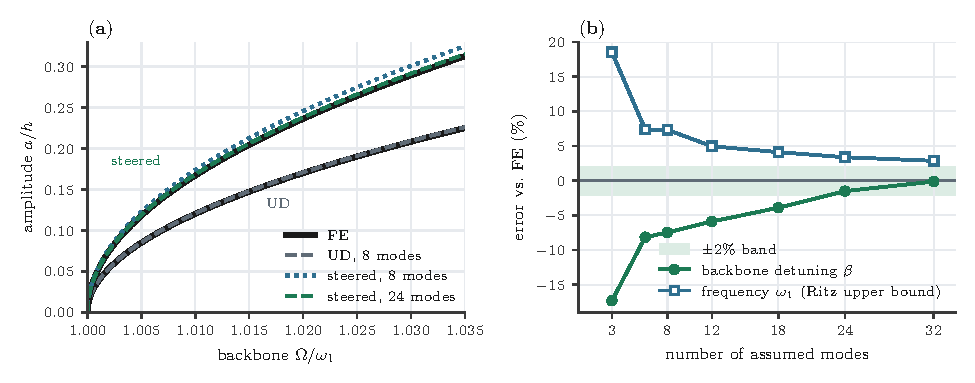
\includegraphics[width=\linewidth]{figs/plate_fe_validation.pdf}
\caption{\textbf{The assumed-modes backbone agrees with an independent finite-element model.}
\textbf{(a)}~Amplitude vs.\ backbone frequency (same orientation as
Figs.~\ref{fig:beam} and \ref{fig:confirm}); black: FE. For the homogeneous UD plate the
8-mode assumed-modes backbone (gray dashed) coincides with FE, validating the FE nonlinear
model; for the strongly steered plate the assumed-modes backbone converges to FE as modes
are added (8 modes dotted, 24 modes green dashed, overlying FE). \textbf{(b)} Ritz convergence toward FE (steered): the normalized
backbone detuning enters the $\pm2\%$ band by $\sim\!24$ modes, whereas the absolute frequency is
a slowly-converging Ritz upper bound. The design quantity (relative detuning) is the well-resolved
one.}
\label{fig:fe}
\end{figure}

Two conclusions. \emph{(i)} For a homogeneous laminate the FE and assumed-modes backbones
agree to $\nFEtabUDagree\%$, validating the FE nonlinear model (membrane, coupling, condensation).
\emph{(ii)} For strong steering the assumed-modes frequency is a Ritz upper bound that
converges slowly, but the \emph{normalized backbone detuning} $\beta\propto\gamma/K_b$
is far more robust --- a ratio of two integrals of the \emph{same} slightly-inaccurate mode, so
the mode-shape error largely cancels, leaving a $\nFEtabDetErrTwentyFour\%$ discrepancy at $24$ modes. The relative
detuning results the designs are built on are therefore FE-accurate to a few percent; absolute
frequencies of strongly steered designs should be read from FE or an enriched
($\gtrsim24$-mode) expansion. The paper's design evaluator uses 64 transverse modes, and the
optimized design itself is evaluated on this FE model in Sec.~\ref{sec:confirm} (detuning
ratio $\nFEratio$ vs.\ $\nCratioSSM$ from the full SSM). A displacement-based von~K\'arm\'an FE would replace the assumed
modes throughout at higher cost, reduced by the same SSM.


\section{Calibration against prior work, and SSM- vs EPMC-driven optimization}\label{app:calib}
We reproduce two published results of \cite{pozzi2025} as a check of the reduction and
its sensitivities, and compare SSM- and EPMC-driven optimization on one benchmark.
\emph{(i)} The backbone sensitivity of two coupled oscillators predicts the perturbed
backbone to within about $3\times10^{-5}$ in $\Om$ over its soften-then-harden shape (the
frequency first falls, then turns back up near an RMS amplitude of 1). Capturing the
turn-back needs a high-order SSM; we use order seven, where \cite{pozzi2025} use order
five with an analytic adjoint (Fig.~\ref{fig:fig2}). The damped eigenvalue
$\lambda=-0.0191\pm0.6177i$ matches exactly. \emph{(ii)} A clamped von K\'arm\'an beam
is shaped by an initial curvature to a prescribed softening backbone, and full-order
EPMC confirms the optimized SSM backbone to $<0.1\%$ (Fig.~\ref{fig:fig3}). Two
departures are noted. First, we use the axially condensed shallow-arch model rather
than a three-DOF-per-node element. Second, we place the target amplitudes inside the
cubic SSM's verified window. Eq.~(33) of \cite{pozzi2025}, taken literally, places a
same-sign quadratic coupling on both masses, which is not energy-consistent; the
potential-derived spring we use leaves the reported eigenvalue unchanged.

\paragraph{Validity window of the cubic SSM.} Over the amplitudes reached by the
full-order EPMC continuation ($a/h\le\nEPMCmaxUD$ for UD, $\le\nEPMCmaxOpt$ for the steered design;
Fig.~\ref{fig:confirm}a), the cubic SSM backbone reproduces the EPMC detuning
$\Om/\omega_1-1$ to within $\nEPMCAgree\%$. The jump thresholds compared in
Sec.~\ref{sec:jumpres} ($a_c/h=\nCUDac$ and $\nCOptac$) lie inside these ranges; we make no
claim beyond them, where higher-order terms bend the true backbone.

\begin{figure}[!tbp]
\centering
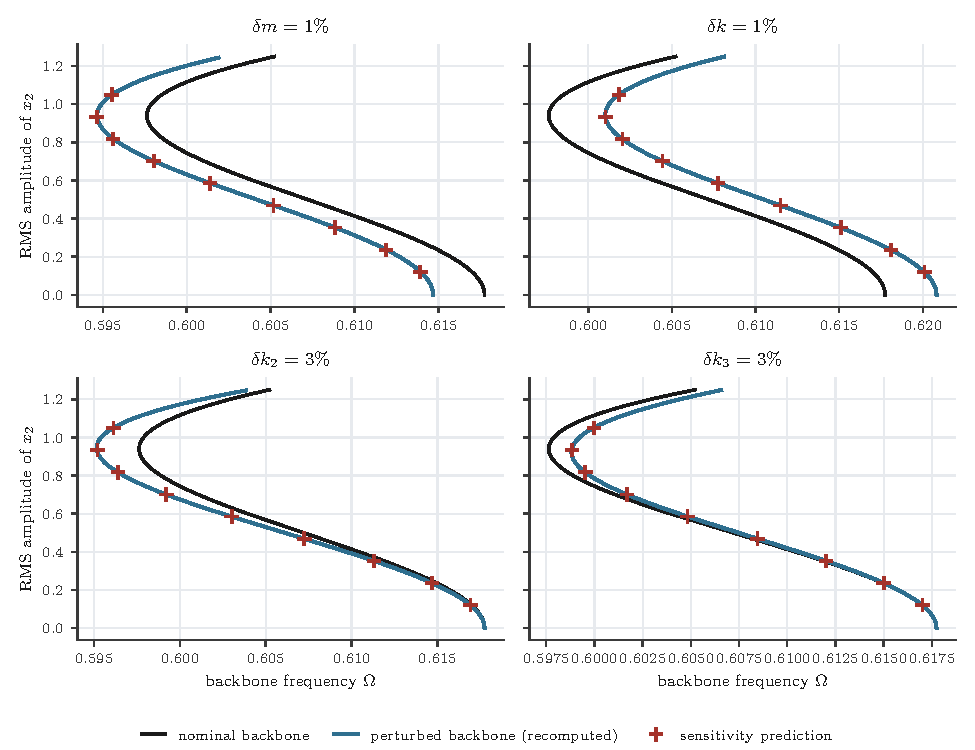
\includegraphics[width=\linewidth]{figs/coupled_osc_sensitivity.pdf}
\caption{\textbf{The backbone sensitivities reproduce a published benchmark.} Calibration against
\cite{pozzi2025}, Fig.~2: backbone-sensitivity
validation of two coupled oscillators. Each panel perturbs one parameter
($m$, $k$: $1\%$; $k_2$, $k_3$: $3\%$). Black: nominal backbone; blue: perturbed backbone,
recomputed; red crosses: first-order sensitivity prediction from the nominal backbone. The
predictions land on the recomputed backbones through the soften-then-harden turn-back,
which the seventh-order SSM captures.}
\label{fig:fig2}
\end{figure}

\begin{figure}[!tbp]
\centering
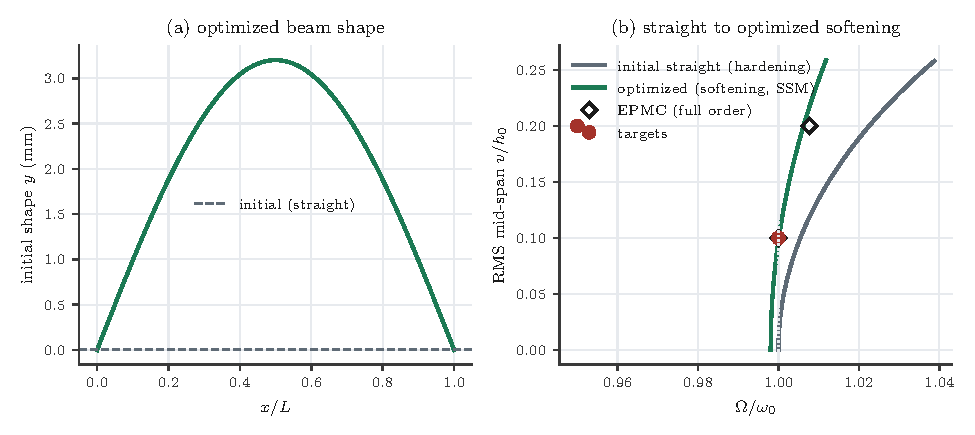
\includegraphics[width=\linewidth]{figs/beam_backbone_opt.pdf}
\caption{\textbf{The SSM design loop reproduces a published backbone-shaping result.} Calibration
against \cite{pozzi2025}, Fig.~3: a von~K\'arm\'an beam
shaped to a prescribed softening backbone. This problem shapes the beam with up to two harmonics (the optimum uses only the first)
to pass through two prescribed backbone points; it is a different problem from that of
Fig.~\ref{fig:svse}, which tunes one amplitude to one target. \textbf{(a)}~Optimized
initial shape $y(x)$ and the straight starting design.
\textbf{(b)}~Backbones, normalized by the first frequency $\omega_{1,0}$ of the initial
straight beam: the straight (hardening) beam becomes a curved (softening) one threading
both target points; full-order EPMC (diamonds) confirms the optimized SSM backbone to
$<0.1\%$.}
\label{fig:fig3}
\end{figure}

\paragraph{EPMC as a design engine.} The extended periodic motion concept
\cite{krack2015} augments the equation of motion with a self-excitation that offsets
damping, $\bm M\ddot{\bm q}+(\bm C-2\delta\Om\bm M)\dot{\bm q}+\bm K\bm q+\bm f_{nl}=\bm0$,
and continues the harmonic-balance residual $\bm R(\bm z;a,\theta)=\bm0$ in amplitude.
Its design sensitivity at a converged point follows from the implicit-function theorem
with the Newton Jacobian already assembled, through one adjoint solve per amplitude,
$\dd\Om/\dd\theta=-\bm w^{\!\top}\partial_\theta\bm R$ with $\bm J_z^{\!\top}\bm w=\bm e_\Om$.
$\partial_\theta\bm R$ reuses the same $\partial\bar{\bm Q}/\partial\theta$ as the SSM
gradient. The two engines are complementary. The SSM gives a smooth, analytic objective
at a cost independent of amplitude and harmonic count, and is the search engine here.
EPMC is exact at any amplitude it reaches, captures folds and internal resonances, and
serves as the validation of record. On the benchmark below, both find nearly the same
optimum, and the SSM backbone is about two orders of magnitude cheaper per evaluation.

\subsection{SSM- and EPMC-driven optimization on the same benchmark}
To compare the two engines as \emph{optimizers}, we solve the same design problem
with each on the published von~K\'arm\'an-beam backbone-shaping benchmark of
\cite{pozzi2025} (their Sec.~5.2 / Fig.~3): a clamped--clamped beam whose backbone
is shaped from hardening to a prescribed \emph{softening} by an initial curvature
$y=A_1\sin(\pi x/L)$. The straight beam hardens ($+2.2\%$ relative detuning at
$\mathrm{RMS}=0.2h_0$); the curvature injects a quadratic nonlinearity whose slaved
response drives the SSM cubic coefficient negative, softening the backbone (it also
stiffens the beam linearly, so the curvature-invariant measure is the detuning
relative to each design's \emph{own} $\omega_1$). We design $A_1$ to hit a $-1.5\%$
softening target, driving the optimizer once with the SSM backbone and once with the
full-order EPMC backbone. Both reach the target exactly. The optima are $A_1=8.03$\,mm
(SSM) and $8.26$\,mm (EPMC), a $2.8\%$ difference that is the cubic SSM's truncation
error at $\mathrm{RMS}=0.2h_0$. The SSM backbone costs about two orders of magnitude less per
evaluation (Fig.~\ref{fig:svse}). This is the intended division of labor: the SSM adjoint does
the search cheaply, and full-order EPMC confirms the optimum.

\begin{figure}[!tbp]
\centering
\begin{minipage}[c]{0.54\linewidth}\centering
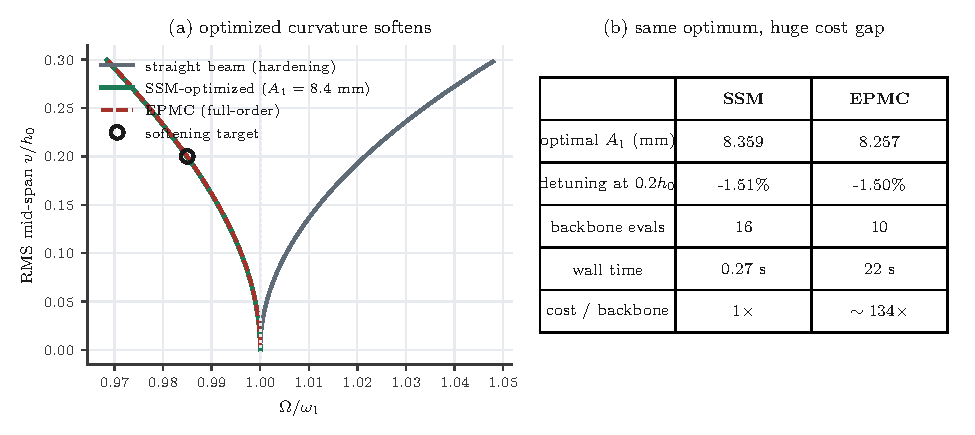
\includegraphics{figs/ssm_vs_epmc_opt.pdf}
\end{minipage}\hfill
\begin{minipage}[c]{0.43\linewidth}\centering\footnotesize
(\textbf{b})\\[4pt]
\IfFileExists{svse_table.tex}{\begin{tabular}{@{}lrr@{}}
\toprule
 & SSM & EPMC\\ \midrule
optimal $A_1$ (mm) & 8.03 & 8.26\\
detuning at $0.2h_0$ & $-1.50\%$ & $-1.50\%$\\
backbone evaluations & 12 & 10\\
wall time (s) & 0.059 & 11.2\\
cost per backbone & $1\times$ & $\approx230\times$\\
\bottomrule
\end{tabular}
}{\textit{table pending}}
\end{minipage}
\caption{\textbf{SSM- and EPMC-driven optimization reach nearly the same optimum, at very different
cost.} Optimizing the same design with both frameworks (benchmark of
\cite{pozzi2025}). Here one curvature amplitude $A_1$ is tuned to one softening
target (a different problem from Fig.~\ref{fig:fig3}). \textbf{(a)}~The straight beam's
backbone hardens (leans right); the
optimized initial curvature softens it (leans left) through the softening target; the
SSM- and EPMC-optimized backbones nearly coincide. \textbf{(b)}~The two optima and
their cost; the SSM optimum differs from the full-order one by the cubic SSM's
truncation error at $\mathrm{RMS}=0.2h_0$, at about two orders of magnitude lower cost
per backbone evaluation (wall times are indicative only).}
\label{fig:svse}
\end{figure}




\section{Verification and reproducibility}\label{app:repro}
Every computed result quoted in the main text and in Appendices A--C is a macro generated
from the result files by \texttt{examples/paper\_numbers.py} (\texttt{docs/paper/numbers.tex}),
or a table written by a listed script; the few rounded bounds and estimates stated in words
(e.g.\ ``less than $0.02$'', the bang-bang estimate $0.4$--$0.5$) follow from those values. The calibration values of Appendix~\ref{app:calib} (the replicated
benchmarks of \cite{pozzi2025}) are printed by the scripts listed for them below. Table~\ref{tab:repro}
maps each result to the script that produces it. Unit tests are in \texttt{tests/}
(\texttt{pytest}).

\begin{table}[!tbp]
\centering\footnotesize
\caption{Result $\to$ script map.}\label{tab:repro}
\begin{tabular}{@{}>{\raggedright\arraybackslash}p{0.42\linewidth}>{\raggedright\arraybackslash}p{0.54\linewidth}@{}}
\toprule
result & script (in \texttt{examples/} unless a path is given)\\ \midrule
relaxed evaluator, gradient, tests & \texttt{nltopt/relaxed\_plate.py}, \texttt{tests/test\_relaxed\_plate.py}\\
beam test (Sec.~\ref{sec:beamres}, Fig.~\ref{fig:beam}) & \texttt{beam\_symmetric\_steering.py}, \texttt{fig\_beam.py}\\
$B$-coupled beam (comparison) & \texttt{steered\_beam\_amplitude\_robust.py}\\
achievable sets (Sec.~\ref{sec:levers}, Fig.~\ref{fig:levers}) & \texttt{levers\_study.py}, \texttt{fig\_levers.py}\\
mechanism, front, dose (Figs.~\ref{fig:mechanism}, \ref{fig:limits}) & \texttt{mechanism\_study.py}, \texttt{fig\_mechanism.py}, \texttt{fig\_limits.py}\\
resolution and pointwise ceiling & \texttt{ceiling\_study.py}\\
full-order confirmation (Sec.~\ref{sec:confirm}), jump (Sec.~\ref{sec:jumpres}) & \texttt{confirm\_heldfreq.py} (SSM, thresholds, sweeps), then \texttt{epmc\_check.py} (merges the EPMC backbones into the same file), \texttt{confirm\_fine\_sweep.py}, \texttt{fig\_confirm.py}\\
independent FE check of the design (Table~\ref{tab:confirm}) & \texttt{fe\_check\_design.py}\\
basis convergence (Table~\ref{tab:conv}) & \texttt{conv\_table.py}\\
continuous-stack competitor (Sec.~\ref{sec:levers}) & \texttt{stack\_continuous.py}\\
frequency multiplier, linear spectra (Secs.~\ref{sec:mechanism}, \ref{sec:discussion}) & \texttt{mechanism\_lambda.py}, \texttt{mode\_ratios.py}\\
all quoted numbers and generated tables & \texttt{paper\_numbers.py}\\
FE validation (App.~\ref{app:fe}) & \texttt{plate\_fe\_backbone.py}, \texttt{plate\_fe\_fig.py}\\
calibration (App.~\ref{app:calib}) & \texttt{coupled\_osc\_sensitivity.py}, \texttt{beam\_backbone\_opt.py}, \texttt{ssm\_vs\_epmc\_opt.py}\\
matched-frequency comparison (Sec.~\ref{sec:confirm}, Fig.~\ref{fig:levers}b) & \texttt{r1\_matched\_frequency.py}\\
other plates, conflict (Sec.~\ref{sec:robust}, Fig.~\ref{fig:robust}a,b) & \texttt{r1\_generality.py}, \texttt{r1\_conflict.py}\\
damping level and law (Fig.~\ref{fig:robust}c) & \texttt{r1\_damping.py}\\
as-built tow defects (Sec.~\ref{sec:asbuilt}, Fig.~\ref{fig:robust}d,e) & \texttt{r1\_asbuilt.py}, \texttt{fig\_robust.py}\\
gradient, independent-grid and multi-start checks (Table~\ref{tab:ms}) & \texttt{r1\_verification.py}\\
\bottomrule
\end{tabular}
\end{table}


\clearpage
\begin{thebibliography}{99}\small
% ---- invariant manifolds, nonlinear normal modes, reduction
\bibitem{shaw} S.\,W.\ Shaw, C.\ Pierre, Normal modes for non-linear vibratory systems,
\emph{J.\ Sound Vib.} 164 (1993) 85--124.
\bibitem{kerschen2009} G.\ Kerschen, M.\ Peeters, J.\,C.\ Golinval, A.\,F.\ Vakakis, Nonlinear
normal modes, Part~I: A useful framework for the structural dynamicist, \emph{Mech.\ Syst.\
Signal Process.} 23 (2009) 170--194.
\bibitem{haller2016} G.\ Haller, S.\ Ponsioen, Nonlinear normal modes and spectral
submanifolds: existence, uniqueness and use in model reduction, \emph{Nonlinear Dyn.} 86
(2016) 1493--1534.
\bibitem{ponsioen2018} S.\ Ponsioen, T.\ Pedergnana, G.\ Haller, Automated computation of
autonomous spectral submanifolds for nonlinear modal analysis, \emph{J.\ Sound Vib.} 420
(2018) 269--295.
\bibitem{jain2022} S.\ Jain, G.\ Haller, How to compute invariant manifolds and their reduced
dynamics in high-dimensional finite element models, \emph{Nonlinear Dyn.} 107 (2022)
1417--1450.
\bibitem{vizzaccaro2022} A.\ Vizzaccaro, A.\ Opreni, L.\ Salles, A.\ Frangi, C.\ Touz\'e, High
order direct parametrisation of invariant manifolds for model order reduction of finite
element structures: application to large amplitude vibrations and uncovering of a folding
point, \emph{Nonlinear Dyn.} 110 (2022) 525--571.
\bibitem{opreni2023} A.\ Opreni, A.\ Vizzaccaro, C.\ Touz\'e, A.\ Frangi, High-order direct
parametrisation of invariant manifolds for model order reduction of finite element
structures: application to generic forcing terms and parametrically excited systems,
\emph{Nonlinear Dyn.} 111 (2023) 5401--5447.
\bibitem{touze} C.\ Touz\'e, A.\ Vizzaccaro, O.\ Thomas, Model order reduction methods for
geometrically nonlinear structures: a review of nonlinear techniques, \emph{Nonlinear Dyn.}
105 (2021) 1141--1190.
\bibitem{krack2015} M.\ Krack, Nonlinear modal analysis of nonconservative systems: extension
of the periodic motion concept, \emph{Comput.\ Struct.} 154 (2015) 59--71.
\bibitem{nayfeh1979} A.\,H.\ Nayfeh, D.\,T.\ Mook, \emph{Nonlinear Oscillations}, Wiley, New
York, 1979.
\bibitem{amabili2008} M.\ Amabili, \emph{Nonlinear Vibrations and Stability of Shells and
Plates}, Cambridge University Press, 2008.
% ---- optimization of nonlinear dynamic response
\bibitem{dou2015} S.\ Dou, B.\,S.\ Strachan, S.\,W.\ Shaw, J.\,S.\ Jensen, Structural optimization
for nonlinear dynamic response, \emph{Phil.\ Trans.\ R.\ Soc.\ A} 373 (2015) 20140408.
\bibitem{doujensen2016} S.\ Dou, J.\,S.\ Jensen, Optimization of hardening/softening behavior
of plane frame structures using nonlinear normal modes, \emph{Comput.\ Struct.} 164 (2016)
63--74.
\bibitem{li2024} M.\ Li, Explicit sensitivity analysis of spectral submanifolds of mechanical
systems, \emph{Nonlinear Dyn.} 112 (2024) 16733--16770.
\bibitem{pozzi2025} M.\ Pozzi, J.\ Marconi, S.\ Jain, M.\ Li, F.\ Braghin, Adjoint sensitivities
for the optimization of nonlinear structural dynamics via spectral submanifolds, \emph{Proc.\
R.\ Soc.\ A} 481 (2025) 20250244.
\bibitem{pozzi2024lsm} M.\ Pozzi, J.\ Marconi, S.\ Jain, F.\ Braghin, Backbone curve tailoring
via Lyapunov subcenter manifold optimization, \emph{Nonlinear Dyn.} 112 (2024) 15719--15739.
\bibitem{pozzi2025smo} M.\ Pozzi, J.\ Marconi, S.\ Jain, M.\ Li, F.\ Braghin, Topology optimization of nonlinear
structural dynamics with invariant manifold-based reduced order models, \emph{Struct.\
Multidiscip.\ Optim.} 68 (2025) 72.
\bibitem{liang2025} H.\ Liang, M.\ Pozzi, J.\ Marconi, S.\ Jain, M.\ Li, Topology optimization of
nonlinear forced response curves via reduction on spectral submanifolds, \emph{Nonlinear Dyn.} 114
(2026) 713.
\bibitem{xiao2026} X.\ Xiao, Using reduced-order models to optimise the dynamics of nonlinear
systems, PhD thesis, University of Bristol, 2026.
\bibitem{kacem2009} N.\ Kacem, S.\ Hentz, D.\ Pinto, B.\ Reig, V.\ Nguyen, Nonlinear dynamics of
nanomechanical beam resonators: improving the performance of NEMS-based sensors,
\emph{Nanotechnology} 20 (2009) 275501.
% ---- composites: laminates, variable stiffness, orientation design
\bibitem{tsai1968} S.\,W.\ Tsai, N.\,J.\ Pagano, Invariant properties of composite materials, in:
\emph{Composite Materials Workshop}, Technomic, 1968, pp.\ 233--253.
\bibitem{hyer1991} M.\,W.\ Hyer, H.\,H.\ Lee, The use of curvilinear fiber format to improve
buckling resistance of composite plates with central circular holes, \emph{Compos.\ Struct.}
18 (1991) 239--261.
\bibitem{gurdal} Z.\ G\"urdal, B.\,F.\ Tatting, C.\,K.\ Wu, Variable stiffness composite panels:
effects of stiffness variation on the in-plane and buckling response, \emph{Compos.\ Part A}
39 (2008) 911--922.
\bibitem{lopes2008} C.\,S.\ Lopes, Z.\ G\"urdal, P.\,P.\ Camanho, Variable-stiffness composite
panels: buckling and first-ply failure improvements over straight-fibre laminates,
\emph{Comput.\ Struct.} 86 (2008) 897--907.
\bibitem{abdalla2007} M.\,M.\ Abdalla, S.\ Setoodeh, Z.\ G\"urdal, Design of variable stiffness
composite panels for maximum fundamental frequency using lamination parameters,
\emph{Compos.\ Struct.} 81 (2007) 283--291.
\bibitem{ijsselmuiden} S.\,T.\ IJsselmuiden, M.\,M.\ Abdalla, Z.\ G\"urdal, Optimization of
variable-stiffness panels for maximum buckling load using lamination parameters, \emph{AIAA
J.} 48 (2010) 134--143.
\bibitem{akhavan2015} H.\ Akhavan, P.\ Ribeiro, Non-linear forced periodic oscillations of
laminates with curved fibres by the shooting method, \emph{Int.\ J.\ Non-Linear Mech.} 76
(2015) 176--189.
\bibitem{akhavan2017} H.\ Akhavan, P.\ Ribeiro, Geometrically non-linear periodic forced
vibrations of imperfect laminates with curved fibres by the shooting method, \emph{Compos.\
Part B} 109 (2017) 286--296.
\bibitem{houmat2013} A.\ Houmat, Nonlinear free vibration of laminated composite rectangular
plates with curvilinear fibers, \emph{Compos.\ Struct.} 106 (2013) 211--224.
\bibitem{yan2021} C.\,A.\ Yan, R.\ Vescovini, E.\,L.\ Jansen, A semi-analytical framework for
nonlinear vibration analysis of variable stiffness plates, \emph{Compos.\ Struct.} 269 (2021)
113954.
\bibitem{farsadi2021} T.\ Farsadi, M.\ Rahmanian, H.\ Kurtaran, Nonlinear lay-up optimization of
variable stiffness composite skew and taper cylindrical panels in free vibration,
\emph{Compos.\ Struct.} 262 (2021) 113629.
\bibitem{farsadi2025} T.\ Farsadi, M.\ Ahmadi, S.\ Jiffri, H.\,H.\ Khodaparast, H.\ Kurtaran, M.\,I.\ Friswell,
S.\ Fichera, Fundamental frequency
optimization of variable stiffness multi-region composite panels in presence of geometrical
nonlinearity, \emph{Mech.\ Syst.\ Signal Process.} 237 (2025) 112972.
\bibitem{zhao2026} R.\ Zhao, Y.\ Yan, K.\ Yu, Y.\ Liu, Nonlinear thermal vibration of variable
stiffness composite laminated plates, \emph{Int.\ J.\ Mech.\ Sci.} 318 (2026) 111527.
\bibitem{pagani2025} A.\ Pagani, A.\ Racionero S\'anchez-Majano, D.\ Zamani, M.\ Petrolo,
E.\ Carrera, Fundamental frequency layer-wise optimization of tow-steered composites
considering gaps and overlaps, \emph{Aerotec.\ Missili Spaz.} 104 (2025) 135--151.
\bibitem{sheikhi2024} M.\ Sheikhi, M.\ Rafiei Anamagh, B.\ Bediz, L.\,T.\ Tunc, Design of
manufacturable variable stiffness composite laminates using spectral Chebyshev and normalized
cut segmentation methods, \emph{Compos.\ Struct.} 330 (2024) 117836.
\bibitem{fayazbakhsh2013} K.\ Fayazbakhsh, M.\ Arian Nik, D.\ Pasini, L.\ Lessard, Defect
layer method to capture effect of gaps and overlaps in variable stiffness laminates made by
automated fiber placement, \emph{Compos.\ Struct.} 97 (2013) 245--251.
\bibitem{kim2012} B.\,C.\ Kim, K.\ Potter, P.\,M.\ Weaver, Continuous tow shearing for
manufacturing variable angle tow composites, \emph{Compos.\ Part A} 43 (2012) 1347--1356.
\bibitem{wu2013} Z.\ Wu, P.\,M.\ Weaver, G.\ Raju, Postbuckling optimisation of variable angle tow
composite plates, \emph{Compos.\ Struct.} 103 (2013) 34--42.
\bibitem{raju2018} G.\ Raju, Z.\ Wu, S.\ White, P.\,M.\ Weaver, Optimal postbuckling design of
variable angle tow composite plates, \emph{AIAA J.} 56 (2018) 2045--2061.
\bibitem{akhavan2018} H.\ Akhavan, P.\ Ribeiro, Aeroelasticity of composite plates with
curvilinear fibres in supersonic flow, \emph{Compos.\ Struct.} 194 (2018) 335--344.
\bibitem{akhavan2020} H.\ Akhavan, P.\ Ribeiro, Stability and bifurcations in oscillations of
composite laminates with curvilinear fibres under a supersonic airflow, \emph{Nonlinear Dyn.}
103 (2021) 3037--3058.
\bibitem{farsadi2019} T.\ Farsadi, D.\ Asadi, H.\ Kurtaran, Nonlinear flutter response of a
composite plate applying curvilinear fiber paths, \emph{Acta Mech.} 231 (2020) 715--731.
\bibitem{akhavan2011} H.\ Akhavan, P.\ Ribeiro, Natural modes of vibration of variable stiffness
composite laminates with curvilinear fibers, \emph{Compos.\ Struct.} 93 (2011) 3040--3047.
\bibitem{ribeiro2012} P.\ Ribeiro, Non-linear free periodic vibrations of variable stiffness
composite laminated plates, \emph{Nonlinear Dyn.} 70 (2012) 1535--1548.
\bibitem{ribeiroakhavan2012} P.\ Ribeiro, H.\ Akhavan, Non-linear vibrations of variable
stiffness composite laminated plates, \emph{Compos.\ Struct.} 94 (2012) 2424--2432.
\bibitem{stegmann2005} J.\ Stegmann, E.\ Lund, Discrete material optimization of general
composite shell structures, \emph{Int.\ J.\ Numer.\ Methods Eng.} 62 (2005) 2009--2027.
\bibitem{nomura2015} T.\ Nomura, E.\,M.\ Dede, J.\ Lee, S.\ Yamasaki, T.\ Matsumori, A.\ Kawamoto,
N.\ Kikuchi, General topology optimization method with continuous and discrete orientation
design using isoparametric projection, \emph{Int.\ J.\ Numer.\ Methods Eng.} 101 (2015)
571--605.
\bibitem{matsuzaki2016} R.\ Matsuzaki, M.\ Ueda, M.\ Namiki, T.-K.\ Jeong, H.\ Asahara, K.\
Horiguchi, T.\ Nakamura, A.\ Todoroki, Y.\ Hirano, Three-dimensional printing of
continuous-fiber composites by in-nozzle impregnation, \emph{Sci.\ Rep.} 6 (2016) 23058.
\bibitem{wong2026} J.\ Wong, E.\,D.\ Sanders, D.\,W.\ Rosen, Toolpath-integrated topology
optimization for design of additively manufactured fiber-reinforced structures considering
limits on fiber curvature, \emph{Compos.\ Struct.} 378 (2026) 119897.
\bibitem{kraft1988} D.\ Kraft, A software package for sequential quadratic programming,
Tech.\ Rep.\ DFVLR-FB 88-28, DLR German Aerospace Center, 1988.
\bibitem{wendland1995} H.\ Wendland, Piecewise polynomial, positive definite and compactly
supported radial functions of minimal degree, \emph{Adv.\ Comput.\ Math.} 4 (1995) 389--396.
\end{thebibliography}

\end{document}
